\documentclass[11pt,a4paper,oldfontcommands,openany]{memoir}
\usepackage{graphicx}
\usepackage[]{color}
\usepackage{courier}
\usepackage[usenames,dvipsnames]{xcolor}
\usepackage[breakable, theorems, skins]{tcolorbox}
\usepackage[]{media9}
\usepackage{lipsum}
\tcbset{enhanced}
%% maxwidth is the original width if it is less than linewidth
%% otherwise use linewidth (to make sure the graphics do not exceed the margin)
\makeatletter
\def\maxwidth{ %
  \ifdim\Gin@nat@width>\linewidth
    \linewidth
  \else
    \Gin@nat@width
  \fi
}
\makeatother

\DeclareRobustCommand{\mybox}[2][gray!15]{%
\begin{tcolorbox}[   %% Adjust the following parameters at will.
        breakable,
        left=0pt,
        right=0pt,
        top=0pt,
        bottom=0pt,
        colback=#1,
        colframe=#1,
        width=\dimexpr\textwidth\relax, 
        enlarge left by=0mm,
        boxsep=5pt,
        arc=0pt,outer arc=0pt,
        ]
        #2
\end{tcolorbox}
}


\definecolor{fgcolor}{rgb}{0.345, 0.345, 0.345}
\newcommand{\hlnum}[1]{\textcolor[rgb]{0.686,0.059,0.569}{#1}}%
\newcommand{\hlstr}[1]{\textcolor[rgb]{0.192,0.494,0.8}{#1}}%
\newcommand{\hlcom}[1]{\textcolor[rgb]{0.678,0.584,0.686}{\textit{#1}}}%
\newcommand{\hlopt}[1]{\textcolor[rgb]{0,0,0}{#1}}%
\newcommand{\hlstd}[1]{\textcolor[rgb]{0.345,0.345,0.345}{#1}}%
\newcommand{\hlkwa}[1]{\textcolor[rgb]{0.161,0.373,0.58}{\textbf{#1}}}%
\newcommand{\hlkwb}[1]{\textcolor[rgb]{0.69,0.353,0.396}{#1}}%
\newcommand{\hlkwc}[1]{\textcolor[rgb]{0.333,0.667,0.333}{#1}}%
\newcommand{\hlkwd}[1]{\textcolor[rgb]{0.737,0.353,0.396}{\textbf{#1}}}%

\usepackage{framed}
\makeatletter
\newenvironment{kframe}{%
 \def\at@end@of@kframe{}%
 \ifinner\ifhmode%
  \def\at@end@of@kframe{\end{minipage}}%
  \begin{minipage}{\columnwidth}%
 \fi\fi%
 \def\FrameCommand##1{\hskip\@totalleftmargin \hskip-\fboxsep
 \colorbox{shadecolor}{##1}\hskip-\fboxsep
     % There is no \\@totalrightmargin, so:
     \hskip-\linewidth \hskip-\@totalleftmargin \hskip\columnwidth}%
 \MakeFramed {\advance\hsize-\width
   \@totalleftmargin\z@ \linewidth\hsize
   \@setminipage}}%
 {\par\unskip\endMakeFramed%
 \at@end@of@kframe}
\makeatother

\definecolor{shadecolor}{rgb}{.97, .97, .97}
\definecolor{messagecolor}{rgb}{0, 0, 0}
\definecolor{warningcolor}{rgb}{1, 0, 1}
\definecolor{errorcolor}{rgb}{1, 0, 0}
\newenvironment{knitrout}{}{} % an empty environment to be redefined in TeX

\usepackage{alltt}
\setlength{\parindent}{0pt} % Remove indent at new paragraphs
\setcounter{secnumdepth}{4}  % Remove section numbering at certain depth # If zero, then no numbering of sections
\setcounter{tocdepth}{4} % Determines number of subsections that will have tabs
\usepackage{tabu}
\usepackage{url}

\usepackage[round]{natbib}   % omit 'round' option if you prefer square brackets
\bibliographystyle{plainnat}

\usepackage{fixltx2e}
%\usepackage{graphicx}	% For external pictures
\usepackage{float}
\usepackage{subfig}	% Add subfigures within figures
\usepackage{verbatim}
\usepackage[colorlinks=true,linkcolor=blue,citecolor=blue,urlcolor=blue]{hyperref}
\usepackage{amssymb,amsbsy,amsmath}
\usepackage{epsfig}
\usepackage[left=3cm,top=3cm,bottom=3.5cm,right=3cm]{geometry} % For easy document margins
%\usepackage{fancyhdr} % For customization of header/footer
\usepackage{adjustbox}
\usepackage{framed}
\usepackage{enumitem}
\usepackage{caption}
\numberwithin{equation}{section} % Equation numbers relative to sections

%%%%% NEW ADDED FROM THESIS.TEX %%%%% 
\usepackage[utf8]{inputenc}
\usepackage[T1]{fontenc}
\usepackage{microtype}
%\usepackage[dvips]{graphicx}
%\usepackage{times} %clash
%%%%%%%%%%%%%%%%%%%%%%%%%%%%%%%%%%%%%%%% 
\newcommand{\code}[1]{{\texttt{#1}}}
\newcommand{\pkg}[1]{{\texttt{#1}}}
\newcommand{\class}[1]{{\textit{#1}}}
\newcommand{\R}{{\normalfont\textsf{R }}{}}
\IfFileExists{upquote.sty}{\usepackage{upquote}}{}


\begin{document}

\sloppy

%%%%%%%%%%%%%%%%%%%%% TITLE PAGE %%%%%%%%%%%%%%%%%%%%%

{
\centering
~\vspace{\fill}

\vspace{2.5cm}

{\LARGE Thesis Proposal}

\vspace{1cm}

{\LARGE\textbf{Visualization methods for genealogical and RNA-sequencing datasets}}

\vspace{1cm}

{\LARGE Lindsay Rutter}

\vspace{4cm}

{\LARGE Program of Study Committee:}

\vspace{1cm}

{\LARGE Dianne Cook (Major Professor)}

\vspace{.25cm}

{\LARGE Amy Toth (Major Professor)}

\vspace{.25cm}

{\LARGE Heike Hofmann}

\vspace{.25cm}

{\LARGE Daniel Nettleton}

\vspace{.25cm}

{\LARGE James Reecy}

\vspace{2.5cm}

{\centerline{\large May 16, 2016}}
}

\clearpage
%\cleardoublepage

%%% CHAPTER'S STYLE
\chapterstyle{bianchi}
\setsecheadstyle{\Large\bfseries\sffamily\raggedright}
\setsubsecheadstyle{\large\bfseries\sffamily\raggedright}
\setsubsubsecheadstyle{\bfseries\sffamily\raggedright}
%%%%%%%%%%%%%%%%%%%%%%%%%%%%%%%%%%%%

\tableofcontents

\setlength{\parskip}{10pt} % Inter-paragraph spacing

%%% ADDED FROM THESIS.TEX %%%%%%%%%
\OnehalfSpacing

\chapter{Introduction}
%%%%%%%%%%%%%%%%%%%%%%%%%%%%%%%%%%%%%%%%%%%%%%%%%%%%%%%%%%%%%%%%%%%
%%%%%%%%%%%%%%%%%%%%%%%%%%%%%%%%%%%%%%%%%%%%%%%%%%%%%%%%%%%%%%%%%%%
\section{Background to data visualization}

The problem with only applying traditional modeling approaches to data is that these models are replete with assumptions that they alone cannot call into question. Fortunately, visualization enables analysts to see things they may not have expected with traditional modeling. By plotting the data, analysts can determine whether or not the applied models are sensible; they can work between visualizations and modeling, enhancing the models based on feedback from the visuals. In sum, graphics are essential for analysts to check the quality of the data, assess the model diagnostics, and compare results from different methods.

%%%%%%%%%%%%%%%%%%%%%%%%%%%%%%%%%%%%%%%%%%%%%%%%%%%%%%%%%%%%%%%%%%%
%%%%%%%%%%%%%%%%%%%%%%%%%%%%%%%%%%%%%%%%%%%%%%%%%%%%%%%%%%%%%%%%%%%
\section{Problems to be addressed}

Genealogical data has a standardized type of display known as a pedigree chart, which we introduce in Chapter \ref{sec:litReview}. While this visual plot is useful for certain genealogical datasets, it is not useful for many genealogical datasets, particularly agricultural ones that are used for breeding purposes. We address this problem by introducing a new type of plot to display the paths between the ancestors and descendants constrained by generation for an individual of interest, which could otherwise not be accomplished with a pedigree chart. This new plot (and other plots) are introduced in Chapter \ref{sec:ggenealogy}.

There are popular plotting tools for analyzing RNA-sequencing data, but there are less popular tools that could be more helfpul for RNA-sequencing analysis. We strive to work on the following five uncommon plotting types that could be useful for better understanding RNA-sequencing data, and we show our work-in-progress toward these goals in Chapters \ref{sec:clustering} and \ref{sec:sigtest}:

\begin{enumerate}
\item \textbf{Parallel coordinate plots}:

In gene expression data analysis, we are striving to find relative patterns. Side-by-side boxplots are often used for this purpose, but they can hide potential problems that could still be lurking in the data after normalization. This is because most RNA-sequencing normalization methods are conducted at the sample-level, and side-by-side boxplots do not show connections between the samples. Consequently, boxplots may deceive analysts to believe that the normalization succeeded in cases where alternative plots (such as parallel coordinate plots) would have otherwise indicated that the normalization was in fact unsuccessful due to the presence of inconsistencies (crossings) between replicates. For this reason, parallel coordinate plots (\citealt{origPCP}, \citealt{origPCP2}) are an essential visual tool when checking the initial normalization process of RNA-sequencing analysis. If the normalization is adequate, then the connections between replications should be flat, and we should only see crossings between treatement groups.

The tools currently available for constructing parallel coordinate plots to assess RNA-sequencing data are severely limited: Namely, the large number of genes present can cause constraints in space and time. With one line being drawn for each gene, our resulting plots will have too many lines being drawn to even view patterns of interest in the first place. Moreover, the construction of these plots can be consuming in computation and time, often requiring analysts to wait for minutes before they can view the output. Even though popular tools to visualize parallel coordinate plots (such as the \code{ggparcoord} function in the \code{GGally} package) can be very useful for many datasets, they are not always helpful for large RNA-sequencing datasets (\citealt{ggally}). As a result, our goal is to develop a new approach that both quickly and meaningfully displays the key pieces of information for RNA-sequencing data with parallel coordinate plots. 

\item \textbf{Pairwise scatterplots}:

We aim to develop visuals that can effectively plot replicates against each other. We can do this by generating pairwise scatterplots for replicates, using the \code{scatmat()} function of the \code{GGally} package (\citealt{ggally}). If the data is high quality, then we would expect negligent differences between read counts across replicates. This would result in a scatterplot where the read counts from the two replicates fall along the x=y relationship. Deviations from this expectation would indicate a quality problem with the data.

With this second goal we face the same challenges that we did with the first goal: We have a plotting algorithm that is not tailored to deal with the vastly sized datasets like RNA-sequencing data. As a result, we again face space (overplotting) and time (computational speed) constraints, and our goal would be to tailor the scatterplot matrix to adapt to large amounts of data. In addition, we must now recognize that the few data points along the perimeter of the x=y relationship that we can see may be misleading. Hence, we would want to develop guidelines in terms of what denotes a high-quality dataset where read counts are similar between replicates and different between treatments. 

\item \textbf{Replicate line plots}:

We aim to build upon a new type of plot for gene expression analysis called the replicate line plot, which was developed fairly recently (\citealt{jds}). This plot can be used to visually mine for genes that have small variability in replicates but large variability across treatments. While this plot has been developed and shown to be useful for two replicates, we would wish to expand upon this so that it can be used for more than two replicates. We show an example from the original study that introduced replicate line plots in Figure \ref{fig:porcupine} (\citealt{jds}).

\begin{figure}[H]
\centering
    \begin{framed}
    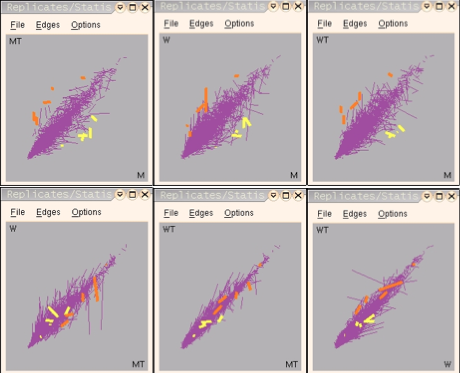
\includegraphics[width=0.8\textwidth]{porcupine}
    \end{framed}
    \caption{Three replicate line plots in which genes of interest (show low variability across replicates but high variability across treatments) are highlighted in orange. For example, in the plot on the left, there are two treatments (MT and M) that each have two replicates. If a gene shows high variability between the two treatments, then it would fall away from the x=y line. If a gene shows low variability between replicates, then the distance between the two replicates will be short. Hence, the genes of interest will be visually represented as the orange ones that are short in length and deviate from the x=y line.}
    \label{fig:porcupine}
\end{figure}

\item \textbf{Single gene plots}:

We plan to develop plots that allow users to look in more detail at individual genes of interest. For instance, while a user may generate a subset of genes from a clustering analysis, they may wish to view the read count across the samples for each of these genes in a visual manner. This may allow a user to quickly sift through the subset of genes and visually determine which ones may truly be of interest.

\item \textbf{Permutation testing plots}:

We aim to develop permutation testing plots for differentially expressed genes. Even if a subset of genes may be deemed statistically significantly differentially expressed, we may wish to see what this might look like if we permuted. We could obtain confidence bands and see if the top differentially expressed genes are signal or noise.

\end{enumerate}

%%%%%%%%%%%%%%%%%%%%%%%%%%%%%%%%%%%%%%%%%%%%%%%%%%%%%%%%%%%%%%%%%%%
%%%%%%%%%%%%%%%%%%%%%%%%%%%%%%%%%%%%%%%%%%%%%%%%%%%%%%%%%%%%%%%%%%%
\section{Overview of thesis research}

%%%%%%%%%%%%%%%%%%%%%%%%%%%%%%%%%%%%%%%%%%%%%%%%%%%%%%%%%%%%%%%%%%%

In Chapter \ref{sec:litReview}, we provide a brief review of the literature behind visualization tools for genealogical data and RNA-sequencing data.

In Chapter \ref{sec:ggenealogy}, we introduce \textbf{\pkg{ggenealogy}} (\citealt{ggen}), a developing \pkg{R} software package that provides tools for searching through genealogical data, generating basic statistics on their graphical structures using parent and child connections, and displaying the results. The package allows users to draw the genealogy in relation to variables related to the nodes, and to determine and display the shortest path distances between the nodes. Production of pairwise distance matrices and genealogical diagrams constrained on generation are also available in the visualization toolkit. We have tested the tools on a dataset with milestone cultivars of soybean varieties (\citealt{soybean}) as well as on a web-based database of the academic genealogy of mathematicians (\citealt{mgp}).

Susan VanderPlas began the original work for this package and developed most features in the \code{plotAncDes()} function. The software package has been available on the Comprehensive \pkg{R} Archive Network since March 2015 (\citealt{ggen}). In August 2015, a paper introducing the \pkg{ggenealogy} software package received a student paper competition award from the Statistical Computing and Graphics Section of the American Statistical Association. Currently, we are preparing to submit another paper describing the software package to the Journal of Statistical Software. We also aim to release a second version of the package as we have added interactive plotting tools that were not available in the first version.

In Chapter \ref{sec:clustering}, we show what we have accomplished toward developing visualization methods for clustering analysis of RNA-sequencing data. We use a soybean example dataset with treatments of iron-poor and iron-rich conditions. On the clustered data, we use both scatterplot matrices and parallel coordinate plots to determine which clusters are of interest. We also use individual gene plots to determine if there subsets of genes within clusters of interest that should be reconsidered.

In Chapter \ref{sec:sigtest}, we demonstrate some of our work-in-progress toward developing visualization methods for significance testing of RNA-sequencing data. We use a paper wasp example dataset with treatments of antennal drumming and nutrition. We use individual transcript plots to determine if the top statistically-significantly differentially expressed transcripts appear to show differences in read counts across the treatments.

In Chapter \ref{sec:timeline}, we tabulate the completed work, the scheduled deliverables for thesis completion, and other work performed outside of thesis work.

\chapter{Literature Review}
\label{sec:litReview}
%%%%%%%%%%%%%%%%%%%%%%%%%%%%%%%%%%%%%%%%%%%%%%%%%%%%%%%%%%%%%%%%%%%
%%%%%%%%%%%%%%%%%%%%%%%%%%%%%%%%%%%%%%%%%%%%%%%%%%%%%%%%%%%%%%%%%%%
\section{Visualization methods for genealogical data}

Publishing in the open source \pkg{R} statistical programming language allows for tools to be distributed and modified at ease, encourages cross-platform collaboration, and provides a foundation for effective and aesthetic data visualization from the grammar of graphics. There are several useful \pkg{R} packages that offer tools for analyzing and visualizing genealogical datasets. Here, we introduce these packages, and emphasize the shortcomings for which our package \pkg{ggenealogy} brings to this collection of work.

The \pkg{R} package \pkg{pedigree} is named after the standardized chart used to study human family lines, and sometimes used to select breeding of animals, such as show dogs (\citealt{ped}). This package does provide tools that perform methods on parent-child datasets, such as rapidly determining the generation count for each member in the pedigree. However, it does not provide any visualization tools.

Another \pkg{R} package called \pkg{kinship2} does produce basic pedigree charts (\citealt{kin}). In Figure \ref{fig:kinshipFig}, we provide an example pedigree chart from the \pkg{kinship2} package vignette. This pedigree chart adheres to the standard set of symbols used for visualizing genealogical structures: Males are represented with squares and females with circles. Parents are connected to each other by horizontal lines, and to their children by vertical lines. Siblings are connected by horizontal sibship lines. Even though this standard pedigree chart creates powerful charts that can be applied across many applications, it cannot provide unequivocal information in situations where inter-generational breeding occurs, as is often the case in agronomic genealogical lineages.

We demonstrate how the standardized pedigree charts in the \pkg{kinship2} package generate ambiguous results in such scenarios by superimposing a hypothetical inter-generational breeding case in Figure \ref{fig:kinshipFig}. In that figure, each generation is defined by its position on the vertical axis, with the first generation containing individuals 201 and 202. We superimposed green-highlighted individual 215 onto the pedigree chart for explanatory purposes. Its parents are individuals 201 and 206, which are from generations one and two, respectively, and have a parent-child relationship between themselves. As an offspring of a parent-child relationship, individual 215 is both a second and third generation individual. Hence, individual 215 should be displayed in both second and third generational positions on the vertical axis. However, standard pedigree tools only allow for an individual to be displayed once. As a result, in special cases where inter-generational breading occurs, such as in agronomic applications, standardized tools for visualizing genealogical information ambiguously portray the genealogical dataset.

\begin{figure}[H]
    \begin{framed}
    \centering
    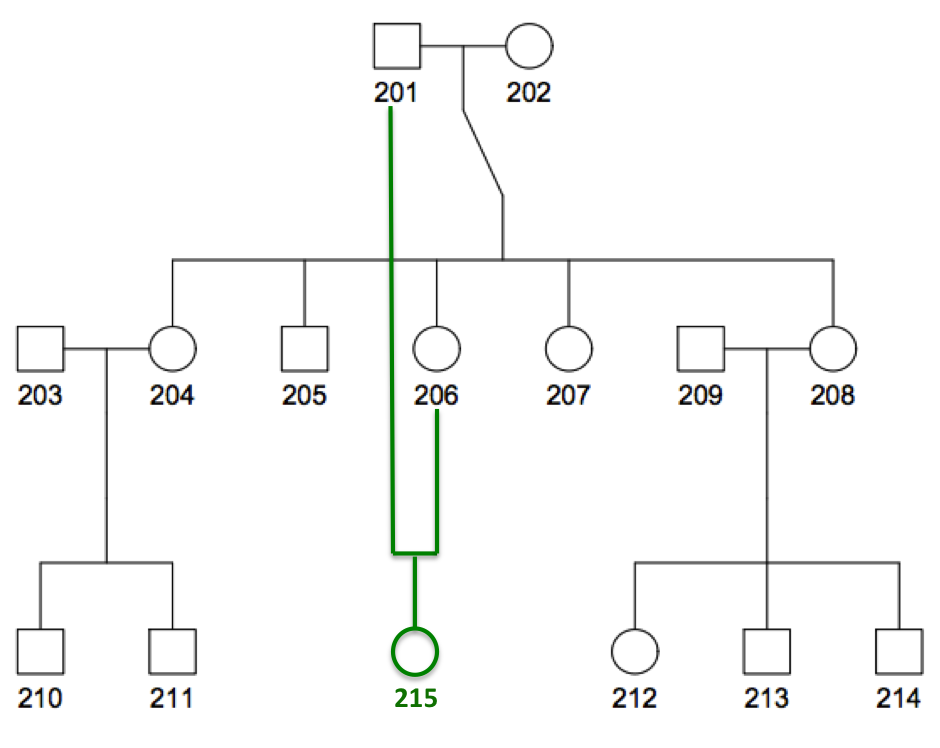
\includegraphics[width=0.65\textwidth]{kinshipFig}
    \end{framed}
    \caption{Example pedigree chart from the \pkg{kinship2} package, where the vertical axis denotes generation count. We superimposed green-highlighted individual 215 for explanatory purposes. As an offspring of a parent-child relationship, individual 215 is both a second and third generation individual. Hence, it should be displayed twice on the vertical axis, once for each of its generation counts. However, standard pedigree tools only allow for an individual to be displayed once, leading to ambiguous portrayal of the genealogical dataset.}
    \label{fig:kinshipFig}
\end{figure}

In addition, popular graph drawing software such as \pkg{GraphViz} and \pkg{Cytoscape} can be used to visualize genealogical structures (\citealt{graphvizCit}, \citealt{cytoscapeCit}). Graphs are defined as objects with sets of nodes and edges, where sets indicate that their comprised elements cannot be repeated. In other words, graphical structures do not allow for repeated nodes, and hence, as is the case with the aforementioned \pkg{R} packages, these popular graph plotting software cannot precisely portray the genealogical dataset in cases of inter-generational breeding.

We again illustrate this problem in Figure \ref{fig:Graph} with an example genealogy using popular graph drawing software like \pkg{GraphViz} and \pkg{Cytoscape}. Here, generation count is denoted by the vertical axis. As was shown in Figure \ref{fig:kinshipFig}, here too we superimpose a green node that has parents from two different generations. This green node is both a second and third generation individual, and should be displayed in both corresponding generation positions on the vertical axis. However, standard graph visualization tools only allow for a given node to be displayed once. As a result, this green node must be ambiguously positioned in either the second or third generation position; in the figure, it is denoted as a third generation individual. In Chapter 3, we will demonstrate \pkg{ggenealogy} plots that can remedy these problems.

\begin{figure}[H]
    \begin{framed}
    \centering
    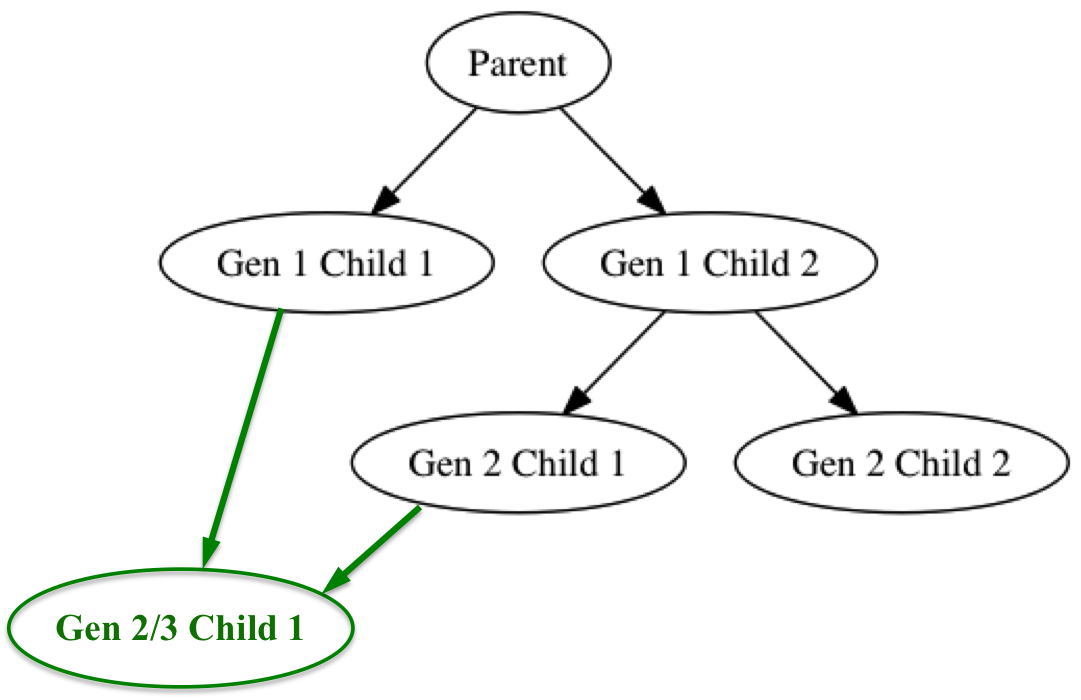
\includegraphics[width=0.6\textwidth]{Graph}
    \end{framed}
    \caption{Example genealogical display using popular graph software like \pkg{GraphViz} and \pkg{Cytoscape}, with generation count denoted by the vertical axis. As was shown in Figure \ref{fig:kinshipFig}, the green node has parents from two different generations, and hence must be ambiguously positioned as one of two generation counts.}
    \label{fig:Graph}
\end{figure}

%%%%%%%%%%%%%%%%%%%%%%%%%%%%%%%%%%%%%%%%%%%%%%%%%%%%%%%%%%%%%%%%%%%
%%%%%%%%%%%%%%%%%%%%%%%%%%%%%%%%%%%%%%%%%%%%%%%%%%%%%%%%%%%%%%%%%%%
\section{Visualization methods for RNA-sequencing data}

Previous studies have provided sound evidence that gene expression data is most effectively explored by using graphical and numerical approaches in a complementary fashion (\citealt{jds}). The authors of this study demonstrated this finding by applying modeling and visualization tools to simulated and real microarray data. Through the use of plots, they determined that their initial models were inappropriate and needed improvement, and that the data quality was questionable and needed relabeling.

Moreover, they demonstrated that some of the most common plots for gene expression data are rife with problems, while some of the less popular plots are useful. In one example, they showed that heatmaps are commonly-used, but they do not allow users to detect outlying genes. In contrast, scatterplots can allow for outlier detection. The authors also showed the importance of interaction on plots for gene expression analysis; they used GGobi (\citealt{ggobi}, \citealt{ggobi2}, \citealt{ggobi3}) to generate direct manipulation and linking between various multivariate plots to display the data. Furthermore, they introduced a new type of plot called the replicate line plot, which can be used to visually mine for genes that show low variability in read counts between replicates but high variablity in read counts between treatments.

%%%%%%%%%%%%%%%%%%%%%%%%%%%%%%%%%%%%%% CHAPTER %%%%%%%%%%%%%%%%%%%%%%%%%%%%%%%%%%%%%% 
%%%%%%%%%%%%%%%%%%%%%%%%%%%%%%%%%%%%%%%%%%%%%%%%%%%%%%%%%%%%%%%%%%%%%%%%%%%%%%%%%%%%%  
 
\chapter{Visualization methods for genealogical datasets}
\label{sec:ggenealogy}

\section{Introduction}

Genealogy is the study of parent-child relationships. By tracing through parent-child lineages, genealogists can study the histories of features that have been modified over time. Comparative geneticists, computational biologists, and bioinformaticians commonly use genealogical tools to better understand the histories of novel traits arising across biological lineages. For example, desirable modifications in crops could include an increase in protein yield or an increase in disease resistance, and genealogical structures could be used to assess how these desirable traits developed. At the same time, genealogical lineages can also be used to assess detrimental features, such as to determine the origin of hazardous traits in rapidly-evolving viruses.

Genealogical structures can also serve as informative tools outside of a strict biological sense. For instance, we can trace mentoring relationships between students and dissertation supervisors with the use of academic genealogies. This can allow us to understand the position of one member in the larger historical picture of academia, and to accurately preserve past relationships for the knowledge of future generations. Similarly, linguistic genealogies can be used to decipher the historical changes of vocabulary and grammatical features across related languages. In short, there is a diverse array of disciplines that can elicit useful information about features of interest by using genealogical data.

In all these examples, the genealogical relationships can be represented visually. Access to various types of plotting tools can allow scientists and others to more efficiently and accurately explore features of interest across the genealogy. We introduce here a developing visualization toolkit that is intended to assist users in their exploration and analysis of genealogical structures. In this paper, we demonstrate the main tools of the software package \pkg{ggenealogy} using two example genealogical datasets, one of soybean cultivars (\citealt{soybean}) and the other of academic mathematicians (\citealt{mgp}).

\section{Example Datasets}
\label{exData}

The \pkg{ggenealogy} package comes with two example datasets, one comprises a soybean genealogy and the other comprises an academic statistician genealogy. We will introduce both example datasets to demonstrate some of the tools available in the software.

\subsection{Soybean Genealogy}

We start with the soybean genealogy, which is available as a data frame structure with 390 rows and five columns. These data were collected from field trials, genetic studies, and United States Department of Agriculture (USDA) bulletins, and date as early as the first decade of the 1900s. They contain information on the copy number variants, single nucleotide polymorphisms, and protein content for each of the varieties, although we removed that information for a succinct example dataset. In this context, the software could ideally be used by agronomists who wish to study how soybean varieties are related. By referencing the visualization of the genealogical structure, these scientists may better understand genetic testing results - in this particular dataset, in terms of copy number variants, single nucleotide polymorphisms, protein content, and yield - and use that knowledge in future breeding decisions.

Each row contains information about a particular child soybean variety, including the name of the child, its yield, the year it was released, whether or not its release year was imputed, and the name of its parent. It should be noted that it typically requires many crosses over the span of one to two decades to develop a new variety that has introduced a desired trait and/or removed an undesired trait. Hence, the release year variable in this dataset represents the year in which the variety was released to the public after its development period. While the name of the child is required, the other four columns can have missing values (which are represented in \pkg{R} with the symbol NA for "not available"). As a result, while each row does contain information about a particular child soybean variety, whether or not a given row also contains information about a parent-child relationship between a pair of soybeans depends on whether or not the parent column has a missing value.

In total, there are 230 soybean varieties in the dataset, 206 of which are children and 165 of which are parents. There are soybeans that are both children and parents. Of the children, 156 have two parents, 28 have one parent, and 22 have zero parents. There are 340 parent-child relationships in the dataset.

We can load the example dataset of soybean genealogy (\code{sbGeneal}) and examine its structure. 

\mybox{
\texttt{R> install.packages("ggenealogy")}\\
\texttt{R> library("ggenealogy")}\\
\texttt{R> data(sbGeneal)}\\
\texttt{R> str(sbGeneal)}
}

\mybox[green!10]{
\texttt{'data.frame':	390 obs. of  5 variables:}\\
\texttt{\$ child       : chr  "5601T" "Adams" "A.K." "A.K. (Harrow)" ...}\\
\texttt{\$ year        : num  1981 1948 1910 1912 1968 ...}\\
\texttt{\$ yield       : int  NA 2734 NA 2665 NA 2981 2887 2817 NA NA ...}\\
\texttt{\$ year.imputed: logi  TRUE FALSE TRUE FALSE FALSE FALSE ...}\\
\texttt{\$ parent      : chr  "Hutcheson" "Dunfield" NA "A.K." ...}
}

\subsection{Academic Genealogy of Statisticians}

The \pkg{ggenealogy} package also comes with an academic genealogy of statisticians; this dataset is in the form of a data frame with 8165 rows and six columns. To develop this later dataset, we contacted the Math Genealogy Project (\citealt{mgp}), a web-based database for the genealogy of academic mathematicians. This database, which currently contains almost 200,000 entries, is a service of the North Dakota State University Department of Mathematics and the American Mathematical Society. The Mathematics Genealogy Project contact provided us a Structured Query Language (SQL) export, and we used PostgreSQL to query the database (\citealt{psql}).

Each entry in the database contained 26 variables pertaining to an individual who received a graduate-level academic degree in mathematics. One of these variables was called "msc" (Mathematics Subject Classification), and we selected only those entries that contained a value of 62 for this variable (coded as "Statistics"). Furthermore, we only retained entries that had a parent if that parent was also in the field of "Statistics". Hence, in our parent-child relationships, both the child and the parent received postbaccalaureate degrees in statistics, and the parent was the academic advisor to the child. This process resulted in 8995 entries, which we reduced to 8165 entries by removing duplicate entries. With the final data frame of 8165 entries, we only maintained six of the original 26 variables. 

Each row of the final data frame contains information about a particular child who received a graduate-level academic degree in statistics, including the name of the child, the year the child obtained the degree, the country and school from which the child obtained the degree, the thesis title of the degree awarded to the child, and the name of its parent. There are no missing values for the country and school from which the child received its degree or the name of the child; however, some of the years contain missing values (NA), and some of the parent and thesis names contain empty strings (""). As a result, while each row does contain information about a particular child, whether or not a row also contains information about a parent-child relationship between a pair of academic statisticians depends on whether or not the parent column has an empty string.
 
In total, there are 7122 individuals in the dataset, 7122 of which are children and 872 of which are parents. Every parent is also a child, but not every child is also a parent. Of the children, two have four parents, ten have three parents, 226 have two parents, 2801 have one parent, and 4083 have no parents. There are 3291 parent-child relationships in the dataset.

We can load the example dataset of academic genealogy of statisticians (\code{statGeneal}) and examine its structure. 

\mybox{
\texttt{R> data(statGeneal)}\\
\texttt{R> dim(statGeneal)}
}

\mybox[green!10]{
\texttt{[1] 8165    6}
}

\mybox{
\texttt{R> colnames(statGeneal)}
}

\mybox[green!10]{
\texttt{[1] "child"   "parent"  "year"    "country" "school"  "thesis"}
}

\section{Genealogical Input Format}

As is the case with both example data files introduced above, \pkg{ggenealogy} requires that the genealogy input file is a data frame structure with at least two columns. One column must be labeled "child", and each case in that column must be of type character. The other column must be labeled "parent," and each case in that column must either be of type character, type NA, or type "". At this point, any \pkg{ggenealogy} plot that only requires information about parent-child relationships can be used.

However, some \pkg{ggenealogy} plots also make use of quantitative variable values associated with individuals in the genealogy. For these plots, the input data frame should also contain a third column. In both example data files, this column is labeled "year," and each case in that column can either be of type numeric, type NA, or type "". At this point, any \pkg{ggenealogy} plot can be used.

\section{Generating a Graphical Object}

Most functions in the \pkg{ggenealogy} software package require an input parameter of a graph structure. Therefore, as a preprocessing step, we must first convert our original data frame structure into a graph structure. Below, we read in the \pkg{R} data file \code{sbGeneal} that is included in the package as a sample data set of soybean genealogy.

We now convert it into an \pkg{igraph} object (\citealt{igraph}) \code{sbIG} using the function \code{dfToIG()}.

\mybox{
\texttt{R> sbIG <- dfToIG(sbGeneal)}\\
\texttt{R> sbIG}
}

\mybox[green!10]{
\texttt{IGRAPH UNW- 230 340 -- }\\
\texttt{+ attr: name (v/c), weight (e/n)}\\
\texttt{+ edges (vertex names):}\\
\texttt{ [1] 5601T    --Hutcheson        Adams    --Dunfield} \\       
\texttt{ [3] A.K.     --A.K. (Harrow)    Altona   --Flambeau} \\       
\texttt{ [5] Amcor    --Amsoy 71         Adams    --Amsoy } \\         
\texttt{ [7] Amsoy 71 --C1253            Anderson --Lincoln   } \\     
\texttt{ [9] Bay      --York             Bedford  --Forrest  }\\       
\texttt{[11] Beeson   --Kent             Blackhawk--Richland } \\      
\texttt{[13] Bonus    --C1266R           Bradley  --J74-39  } \\       
\texttt{[15] Bragg    --Jackson          Bragg    --Bragg x D60-7965}\\
\texttt{+ ... omitted several edges}
}

There are many statistics about the \code{sbGeneal} dataset that we may wish to know that cannot easily be obtained through images and tables. The package function \code{getBasicStatistics()} can be called, using the \code{sbIG} object as input. This will return a list of common graph theoretical measurements regarding the genealogical structure. For instance, is the whole structure connected? If not, how many separated components does it contain? In addition to these statistics, the \code{getBasicStatistics()} function will also return the number of nodes, the number of edges, the average path length, the graph diameter, and other graph theoretical information.

\mybox{
\texttt{R> getBasicStatistics(sbIG)}
}

\mybox[green!10]{
\texttt{\$isConnected}\\
\texttt{[1] FALSE}\\

\texttt{\$numComponents}\\
\texttt{[1] 11}\\

\texttt{\$avePathLength}\\
\texttt{[1] 5.333746}\\

\texttt{\$graphDiameter}\\
\texttt{[1] 13}\\

\texttt{\$numNodes}\\
\texttt{[1] 230}\\

\texttt{\$numEdges}\\
\texttt{[1] 340}\\

\texttt{\$logN}\\
\texttt{[1] 5.438079}
}

\section{Plotting a Shortest Path}

With soybean lineages, it may be useful for soybean breeders to track how two varieties are related to each other via parent-child relationships. Then, any dramatic changes in yield and other measures of interest between the two varieties can be traced across their genetic timeline. The \pkg{ggenealogy} package allows users to select two varieties of interest, and determine the shortest pathway of parent-child relationships between them, using the \code{getPath()} function. This will return a list that contains the variety names and their years in the path.

\mybox{
\texttt{R> pathTN <- getPath("Tokyo", "Narow", sbIG, sbGeneal)}\\
\texttt{R> pathTN}
}

\mybox[green!10]{
\texttt{\$pathVertices}\\
\texttt{[1] "Tokyo"    "Volstate" "Jackson"  "R66-873"  "Narow"}\\   

\texttt{\$yearVertices}\\
\texttt{[1] "1907"   "1942"   "1954.5" "1971.5" "1985"}
}

The returned path object can then be plotted using the \code{plotPath()} function.

\mybox{
\texttt{R> plotPath(pathTN)}
}

\begin{figure}[h]
    \begin{framed}
    \centering
    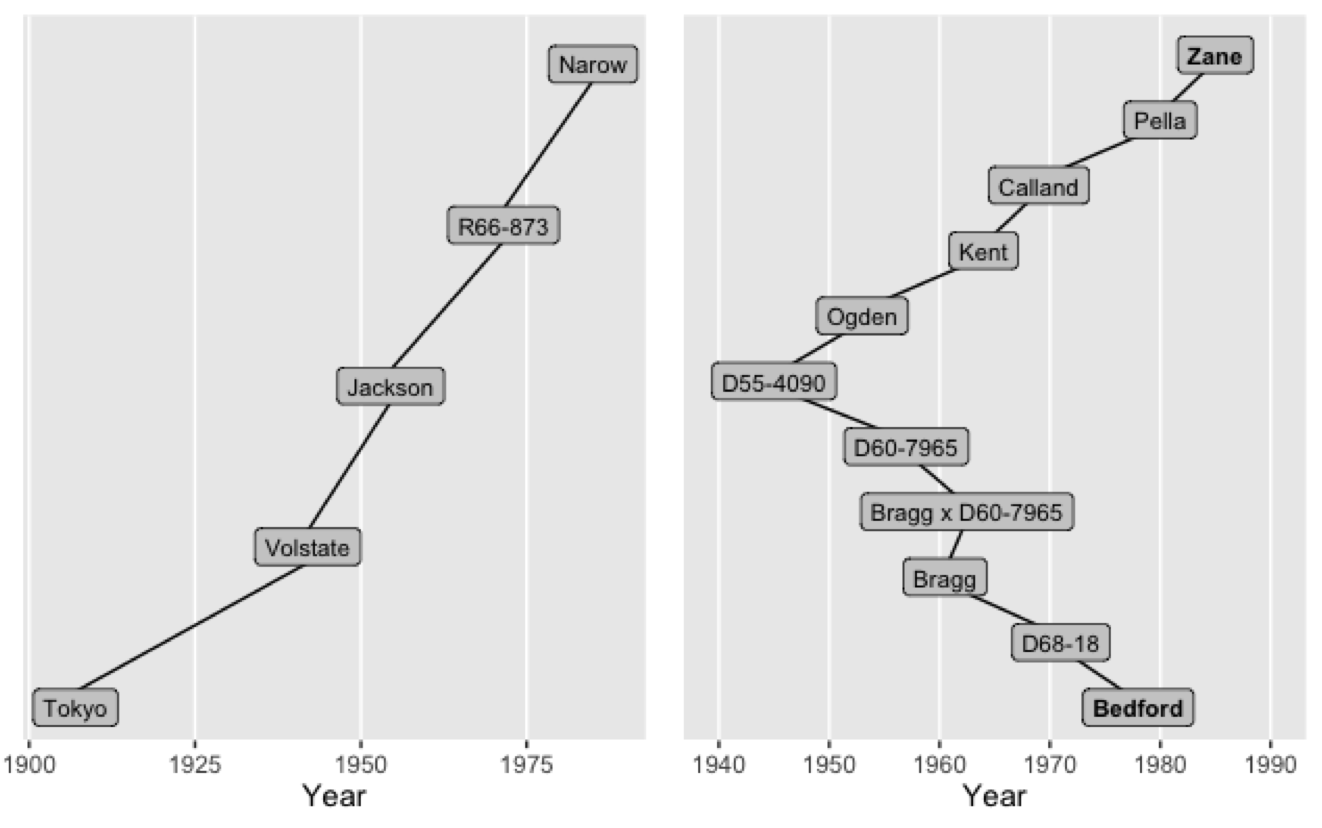
\includegraphics[width=\textwidth]{pathTNZB}
    \end{framed}
    \caption{Left: The shortest path between varieties Tokyo and Narow is strictly composed of a unidirectional sequence of parent-child relationships. Right: The shortest path between varieties Zane and Bedford is not strictly composed of unidirectional parent-child relationships; they instead have a cousin-like relationship.}
    \label{fig:pathTNZB}
\end{figure}

This produces a visual that informs users of all the varieties involved in the shortest path between the two varieties of interest (see left half of Figure \ref{fig:pathTNZB}). In this plot, the release year of all varieties involved in the path are indicated on the horizontal axis, while the vertical axis has no meaning other than to simply to display the labels evenly spaced vertically. The shortest path between varieties \code{Tokyo} and \code{Narow} is composed of a unidirectional series of parent-child relationships, with \code{Tokyo} as the starting ancestor in the early 1900s, \code{Narow} as the most recent descendent in the mid 1980s, and three varieties in between.

Next, we can run the same set of functions on a different pair of varieties. First, a call to the \pkg{ggenealogy} function \code{getYear()} indicates that variety \code{Bedford} was released in 1978 and variety \code{Zane} in 1985.

\mybox{
\texttt{R> getYear("Bedford", sbGeneal)}
}

\mybox[green!10]{
\texttt{[1] 1978}
}

\mybox{
\texttt{R> getYear("Zane", sbGeneal)}
}

\mybox[green!10]{
\texttt{[1] 1985}
}

We can then create a plot showing the shortest path between these two varieties of interest. As this is a longer path, we may also consider setting the \code{fontFace} variable of the \code{plotPath()} to a value of 2, indicating we wish to boldface the two varieties of interest.

\mybox{
\texttt{R> pathBZ <- getPath("Bedford", "Zane", sbIG, sbGeneal)}\\
\texttt{R> plotPath(pathBZ, fontFace = 2)}
}

The resulting plot (right half of Figure \ref{fig:pathTNZB}) allows us to quickly determine that \code{Bedford} is not a parent, grandparent, or any great grandparent of \code{Zane}. Instead, we see that these two varieties are not related through a unidirectional parent-child lineage, but instead have a cousin-like relationship. The oldest common ancestor between \code{Zane} and \code{Bedford} is the variety \code{D55-4090}, which was released in the mid 1940s.

Furthermore, as determined by the figure, for both \code{Zane} and \code{Bedford}, there are four varieties of unidirectional parent-child relationships between each of them and their common ancestor \code{D55-4090}. Hence, any feature of interest that differentiates \code{Zane} and \code{Bedford} (protein content, yield, disease resistance, etc.) can also be examined across these two separate lineage histories.

\section{Superimposing Shortest Path on Tree}

Now that we can create path objects, we may wish to know how those paths are positioned compared to the entire genealogical lineage. For instance, of the documented soybean cultivar lineage varieties, where does the shortest path between two varieties of interest exist? Are these two varieties older compared to the overall data structure? Are they newer? Or, do they span the entire structure, and represent two extreme ends of documented time points?

There is a function available in the \pkg{ggenealogy} package \code{plotPathOnAll()} that can allow users to quickly visualize their path of interest superimposed over all varieties and edges present in the whole data structure. Here we will produce a plot of the shortest path between varieties \code{Tokyo} and \code{Narow} across the entire dataset, as is displayed in Figure \ref{fig:plotTNBin3}.

\mybox{
\texttt{R> plotPathOnAll(pathTN, sbGeneal, sbIG, binVector = 1:3, pathEdgeCol = "red", nodeSize = 2.5, pathNodeSize = 4) + ggplot2::theme(axis.text = ggplot2::element\_text(size = 12), axis.title = ggplot2::element\_text(size = 12))}
}

\begin{figure}%[h]
    \begin{framed}
    \centering
    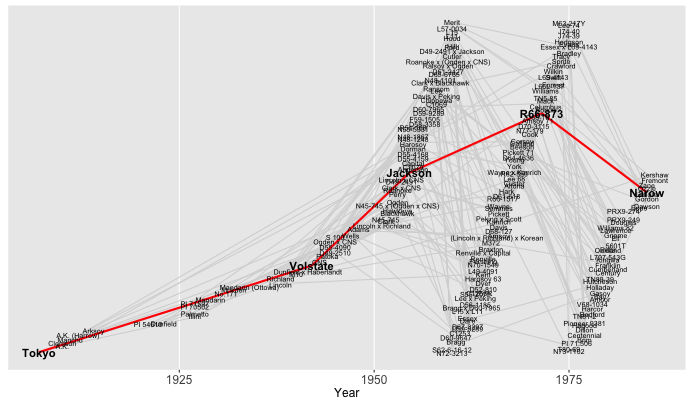
\includegraphics[width=\textwidth]{plotTNBin3}
    \end{framed}
    \caption{The shortest path between Tokyo and Narow, superimposed over the data structure, using a bin size of 3.}
    \label{fig:plotTNBin3}
\end{figure}

In the code above, syntax from the \pkg{ggplot2} package was appended to the \code{plotPathOnAll()} function; this can be done for most \pkg{ggenealogy} functions (\citealt{ggplot2}). While the first three explicit parameters have been introduced earlier in this paper, the fourth parameter (\code{binVector}) requires some explanation. The motivation of the \code{plotPathOnAll()} function is to write node labels on a plot, with the center of each node label constricted on the horizontal axis to its quantitative variable of interest (in this case, year of release). As is the case for the plots before, the vertical axis has no meaning other than providing a plotting area in which to draw the node labels. Unfortunately, for large datasets, this motivation can be a difficult task because the text labels of the varieties can overlap if they are assigned a similar y coordinate, have a similar year (x coordinate), and have long text labels (width of x coordinate).

For each variety, the x coordinate (year) and width of the x coordinate (text label width) cannot be altered, as they provide useful information. However, for each variety, the y coordinate is arbitrary. Hence, in an attempt to mitigate text overlapping, the \code{plotPathOnAll()} function does not randomly assign the y coordinate. Instead, it allows users to partially control the y coordinates with a user-determined number of bins (\code{binVector}).

If the user decides to produce a plot using three bins, as in the example code above, then the varieties are all grouped into three bins based on their year values. In other words, there will be bin 1 (the "oldest bin") which includes the one-third of varieties with the oldest years of release, bin 2 (the "middle bin"), and bin 3 (the "youngest bin"). Then, in order to decrease text overlap, the consecutively increasing y-axis coordinates are alternatively assigned to the three bins (For example: bin 1, bin 2, bin 3, bin 1, bin 2, bin 3, ...) repeatedly until all varieties are addressed. This algorithm means that for any pair of varieties within a given bin, there are exactly two other varieties vertically separating them.

In the code above, \code{binVector} was assigned a value of 3, and \code{pathEdgeCol} was assigned a value of "red". Additionally, we specified a size of 2.5 for the non-path node test using the \code{nodeSize} parameter, and a size of 4 for the path node text using the \code{pathNodeSize} parameter. There are several other parameters in the \code{plotPathOnAll()} function, which can be read in more detail using the help command.

This code resulted in Figure \ref{fig:plotTNBin3}, where we see that edges not on the path of interest are thin and gray by default, whereas edges on the path of interest are bolded by default. We also see that variety labels in the path of interest are boldfaced by default. Figure \ref{fig:plotTNBin3} presents useful information: We immediately gather that the path of interest does span most of the years of the data structure. In fact, \code{Tokyo} appears to be the oldest variety in the dataset, and \code{Narow} appears to be one of the youngest varieties. We can also determine that the majority of varieties were released between 1950 and 1970.

However, Figure \ref{fig:plotTNBin3} has significant empty spaces between the noticeably distinct bins, whereas almost all text labels are overlapping, thereby decreasing their readability. To force text labels into these spaces, the user may consider using a larger number of bins. Hence, we next examine a bin size of 6 to create Figure \ref{fig:plotTNBin6}.

\mybox{
\texttt{R> plotPathOnAll(pathTN, sbGeneal, sbIG, binVector = 1:6, pathEdgeCol = "seagreen2", nodeSize = 1, pathNodeSize = 3)}
}

\begin{figure}[H]
    \begin{framed}
    \centering
    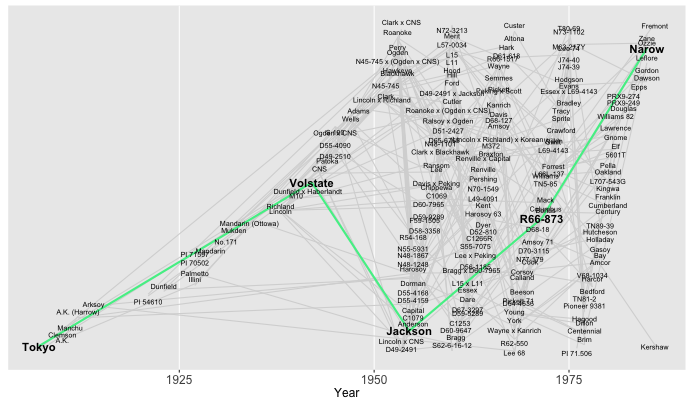
\includegraphics[width=\textwidth]{plotTNBin6}
    \end{framed}
    \caption{The shortest path between Tokyo and Narow, superimposed over the data structure, using a bin size of 6.}
    \label{fig:plotTNBin6}
\end{figure}

We can immediately see that Figure \ref{fig:plotTNBin6} more successfully mitigates text overlap compared to Figure \ref{fig:plotTNBin3}. We can also confirm what we saw in the previous plot that indeed most varieties were released between 1950 and 1970, and any textual overlap is confined to this range of years.

\section{Plotting Ancestors and Descendants by Generation}
\label{remedy}

The most novel visual function in \pkg{ggenealogy}, \code{plotAncDes()} allows users to view the ancestors and descendants of a given variety. The inputted variety is highlighted in the center of the plot, ancestors are displayed to the left of the center, and descendants are displayed to the right of the center. The further from the center that a variety is located, the more generations that variety is distanced from the centered variety of interest.

This particular \pkg{ggenealogy} tool is unique because most available genealogy and graph visualization software do not allow for repeated labels. It is a useful tool because, as was demonstrated in Figures \ref{fig:kinshipFig} and \ref{fig:Graph}, some genealogical datasets require repeated node labels if they are to be visualized by generation counts. Indeed, our example soybean genealogy is one such dataset.

To demonstrate this tool, we will create a plot of the ancestors and descendants of the variety \code{Lee}. We specify that the maximum number of ancestor and descendant generations are both 6, and that the text of the variety of interest is highlighted in blue:

\mybox{
\texttt{R> plotAncDes("Lee", sbGeneal, mAnc = 6, mDes = 6, vCol = "blue")}
}

This generates the top plot of Figure \ref{fig:Lee}. We notice that \code{Lee} has 3 generations of ancestors and 5 generations of descendants. We also notice that some varieties are repeated in the plot, which is a unique feature provided by \pkg{ggenealogy}. For example, the variety \code{5601T} is represented four times - once as a third generation descendant of \code{Lee}, once as a fourth generation descendant of \code{Lee}, and twice as a fifth generation descendant of \code{Lee}. The variety \code{5601T} was repeated multiple times because there are multiple paths between \code{Lee} and \code{5601T}. For explanation purposes, all paths between \code{Lee} and \code{5601T} were manually highlighted in blue.

\begin{figure}[H]
    \begin{framed}
    \centering
    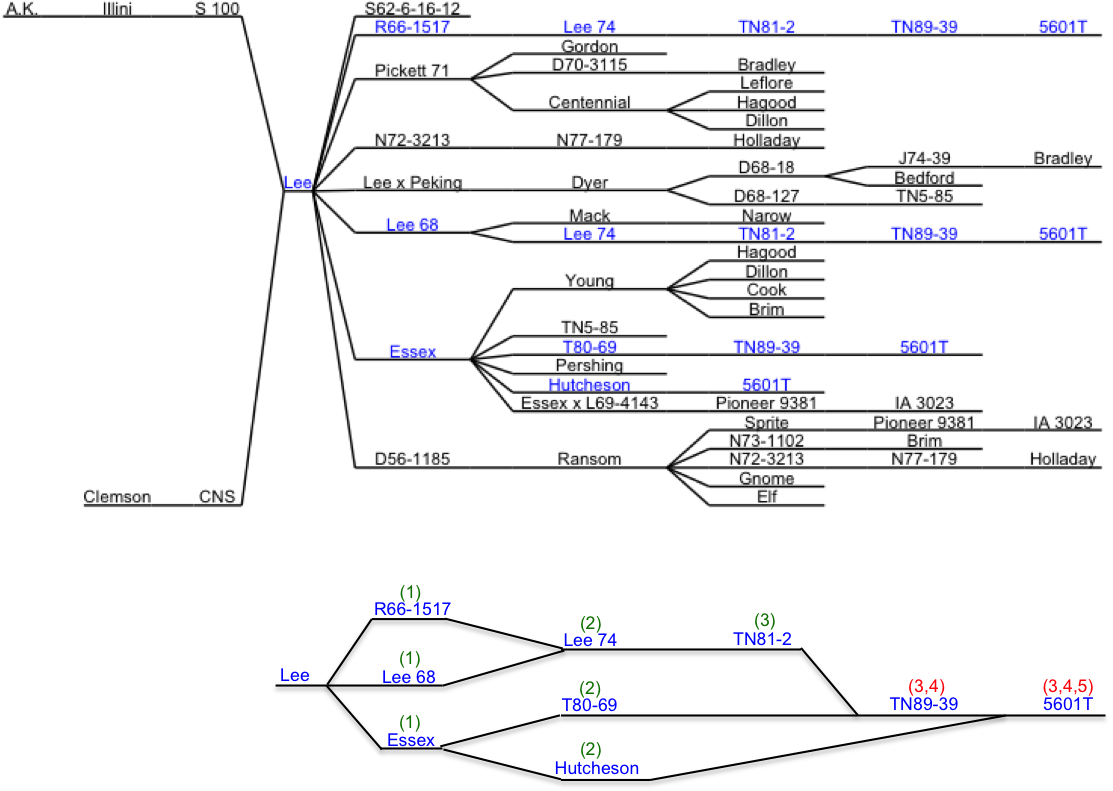
\includegraphics[width=\textwidth]{LeeAD3}
    \end{framed}
    \caption{Top: All ancestors and descendants of the variety Lee are shown in this ggenealogy plot. Bottom: We now attempt to mimic the blue paths in the ggenealogy plot on the top, only now nodes cannot be repeated. The parenthetical numbers above each node represents the set of generation counts that node is away from the center node Lee. The presence of red parentheses indicate that the plot on the bottom ambiguously display the example soybean genealogy in the way that the ggenealogy plot on the top can accomplish.}
    \label{fig:Lee}
\end{figure}

The bottom plot of Figure \ref{fig:Lee} is not an output plot of \pkg{ggenealogy}. Instead, it was simply created for didactic purposes. Here, the paths that were manually highlighted in blue in the top plot produced by \pkg{ggenealogy} are shown again, only now nodes cannot be repeated. The parenthetical number above each node represents the set of generation counts distancing that node from the center node \code{Lee}; green parentheses indicate that the node could be successfully placed in one horizontal position, but red parentheses indicate that the node could not be successfully placed in one horizontal position. We see that node \code{TN89-39} cannot simultaneously be represented as both a third and fourth descendent of node \code{Lee}, and node \code{5601T} cannot simultaneously be represented as a third, fourth, and fifth descendent of node \code{Lee}. Hence, without allowing nodes to repeat, this dataset cannot be presented in the graph on the bottom as it can be in the \pkg{ggenealogy} graph on the top. This is a current limitation in other genealogy and graphical software that \pkg{ggenealogy} can now provide.

\section{Plotting Distance Matrix}

It may also be of interest to generate matrices where the colors indicates a variable between all pairwise combinations of inputted varieties. The package \pkg{ggenealogy} also provides a function \code{plotDegMatrix()} for that purpose. We can demonstrate this function with the variable being the shortest path degree between a given pair of varieties. The shortest path degree is calculated as the smallest number of parent-child edges needed to traverse between two varieties of interest. For instance, in Figure \ref{fig:pathTNZB}, the shortest path degree between \code{Tokyo} and \code{Narow} is four and the shortest path degree between \code{Bedford} and \code{Zane} is ten.

Here we generate a distance matrix for a set of 10 varieties, setting the x-label and y-label as "Variety" and the legend label as "Degree". In this example, we add \pkg{ggplot2} functionality to specify that pairs with small degrees are white, while those with large degrees are dark green, as well as to specify the text size of the legend title and label.

\mybox{
\texttt{>R varieties <- c("Brim", "Bedford", "Calland", "Dillon", "Hood", "Narow", "Pella", "Tokyo", "Young", "Zane")}\\
\texttt{>R plotDegMatrix(varieties, sbIG, sbGeneal, "Variety", "Variety", "Degree") + ggplot2::scale\_fill\_continuous(low = "white", high = "darkgreen") + ggplot2::theme(legend.title = ggplot2::element\_text(size = 15), legend.text = ggplot2::element\_text(size = 15))}
}

This creates the plot in Figure \ref{fig:degMatrix}. We see that the degree of the shortest path between varieties \code{Bedford} and \code{Zane} is 10, which is consistent with what we saw earlier in Figure \ref{fig:pathTNZB}. However, we now also see that a shortest path degree of 10 may be considered relative to the rest of this dataset.

\begin{figure}[h]
    \begin{framed}
    \centering
    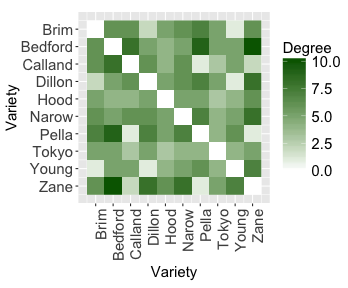
\includegraphics[width=0.5\textwidth]{degMatrix}
    \end{framed}
    \caption{The shortest path degree matrix between ten varieties of interest.}
    \label{fig:degMatrix}
\end{figure}

\section{Academic Genealogy of Statisticians}

The \pkg{ggenealogy} package comes with two example datasets, and while we have introduced the plant breeding genealogy, we have yet to introduce the academic genealogy. As was demonstrated in Section \ref{exData}, every parent in the academic genealogy is also a child, and some children in the academic genealogy have more than two parents. Neither of these features was the case in the plant breeding genealogy. Additionally, the academic genealogy is much larger than the plant breeding genealogy. Some of these differences may affect how one would approach \pkg{ggenealogy} plotting tools. For this reason, we will now demonstrate some of the \pkg{ggenealogy} plotting tools we already introduced, only now applied to the academic genealogy. 

The ability to plot ancestors and descendants by generation was demonstrated using the plant breeding genealogy in Figure \ref{fig:Lee}. As we believe this is the most novel plotting tool in the \pkg{ggenealogy} package, we will test it again here using the academic genealogy.

We need to choose a central individual of interest in order to create this plot. Perhaps we can use the academic statistician in the dataset that has the largest number of "descendants". To determine the name of this individual, below we use the \pkg{ggenealogy} function \code{getNode()} to create a vector \code{indVec} that contains the names of all individuals in the dataset. We then use the \pkg{dplyr} package to apply the \pkg{ggenealogy} function \code{getDescendants()} on each individual in the \code{indVec} vector (\citealt{dplyr}). We set the parameter \code{gen} to a conservatively large value of 100 as this dataset is unlikely to have any individuals with more than 100 generations of "descendants".

After that, we can generate a table to examine all values of "descendant" counts in the dataset, along with the number of individuals who have each of those values of "descendant" counts. Of the 8165 individuals in this dataset, 6252 of them have zero "descendants", 322 of them have one "descendant", and 145 of them have two "descendants". There are only 17 individuals who have more than 30 "descendants", and there is one individual who has the largest value of 159 "descendants". We determine that this individual is the prominent British statistician Sir David Cox, who is known for the Box-Cox transformation and Cox processes, as well as for mentoring many younger researchers who later became notable statisticians themselves.

\mybox{
\texttt{>R library(dplyr)}\\
\texttt{>R indVec <- getNodes(statGeneal)}\\
\texttt{>R indVec <- indVec[which(indVec != "", )]}\\
\texttt{>R dFunc <- function(var) nrow(getDescendants(var, statGeneal, gen = 100))}\\
\texttt{>R numDesc <- sapply(indVec, dFunc)}\\
\texttt{>R table(numDesc)}
}

\mybox[green!10]{
\texttt{numDesc}\\
\texttt{   0    1    2    3    4    5    6    7    8    9   10   11   12   13   14 }\\
\texttt{6252  322  145   88   58   36   31   22   23   14   17   13   14    9    9 }\\
\texttt{  15   16   17   18   19   20   21   22   23   24   25   26   27   29   30 }\\
\texttt{   6    4    3    2    5    7    5    3    3    2    2    6    1    1    3 }\\
\texttt{  34   37   38   40   41   44   45   48   49   61   62   75   77   84  159 }\\
\texttt{   2    1    1    1    1    1    1    1    2    1    1    1    1    1    1 }
}

\mybox{
\texttt{R> which(numDesc == 159)}
}

\mybox[green!10]{
\texttt{David Cox}\\ 
\texttt{     1980}
}

We can now visualize how these 159 "descendants" are related to Sir David Cox by calling the \code{plotAncDes()} function of \pkg{ggenealogy}, similar to what we did to generate Figure \ref{fig:Lee}. As such, we create Figure \ref{fig:dCox} using the code below.

\mybox{
\texttt{R> plotAncDes("David Cox", statGeneal, mAnc = 6, mDes = 6, vCol = "blue")}
}

\begin{figure}%[h]
    \begin{framed}
    \centering
    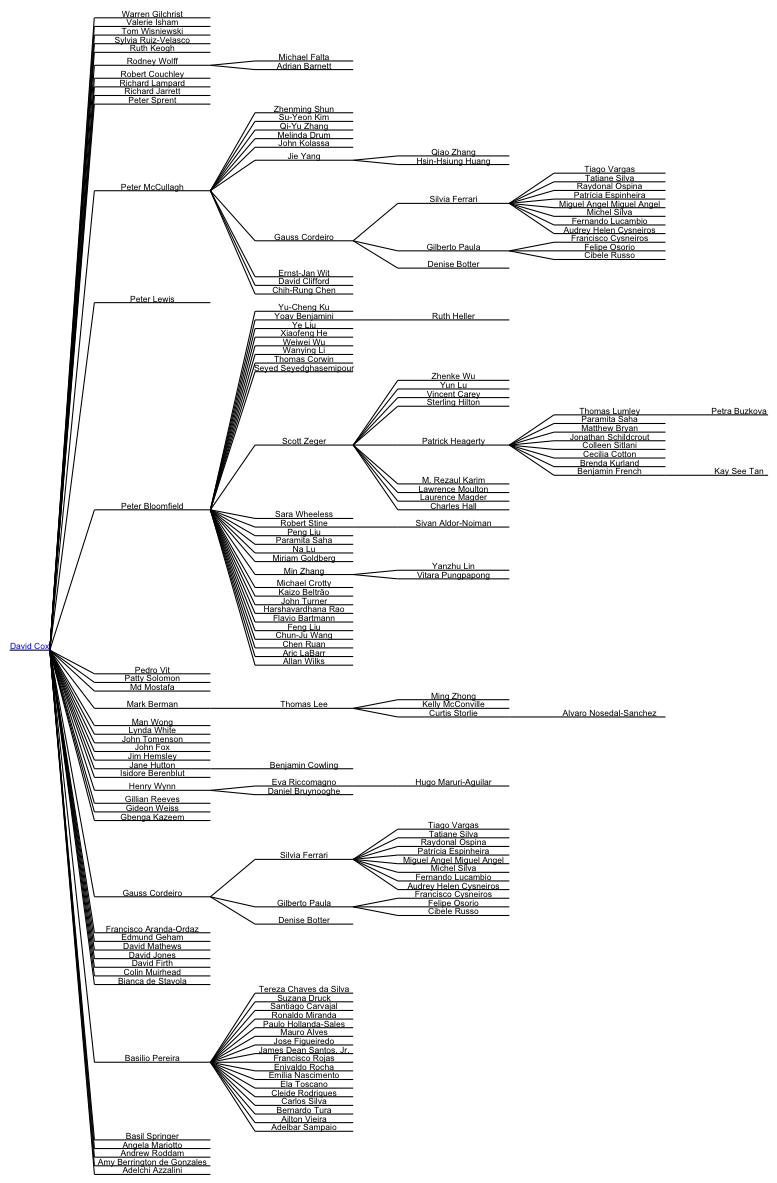
\includegraphics[width=\textwidth]{dCox.png}
    \end{framed}
    \caption{The 159 academic statistician "descendants" of Sir David Cox.}
    \label{fig:dCox}
\end{figure}

We see from Figure \ref{fig:dCox} that Sir David Cox had 42 "children", many of them becoming notable statisticians themselves, such as Basilio Pereira, Valerie Isham, Gauss Cordeiro, Peter McCullagh, and Henry Wynn. Of his "children", the one who produced the most "children" of their own was Peter Bloomfield, who has 26 "children" and 49 "descendants". In total, Sir David Cox had five generations of academic statistics mentees in this dataset.

\mybox{
\texttt{R> length(getChild("Peter Bloomfield", statGeneal))}
}

\mybox[green!10]{
\texttt{[1] 26}
}

\mybox{
\texttt{R> nrow(getDescendants("Peter Bloomfield", statGeneal, gen = 100))}
}

\mybox[green!10]{
\texttt{[1] 49}
}

At this point, it would be insightful to examine a more detailed view of one of the longest strings of "parent-child" relationships between Sir David Cox and one of the two individuals who are his fifth generation "descendants". We do so with the code below, choosing his fifth generation "descendant" to be Petra Buzkova. We set the \code{fontFace} variable of the \code{plotPath()} to a value of 4, indicating we wish to boldface and italicize the two varieties of interest.

\mybox{
\texttt{R> statIG <- dfToIG(statGeneal)}\\
\texttt{R> pathCB <- getPath("David Cox", "Petra Buzkova", statIG, statGeneal, isDirected = FALSE)}\\
\texttt{R> plotPath(pathCB, fontFace = 4) + ggplot2::theme(axis.text = ggplot2::element\_text(size = 10), axis.title = ggplot2::element\_text(size = 10))}
}

\begin{figure}[H]
    \begin{framed}
    \centering
    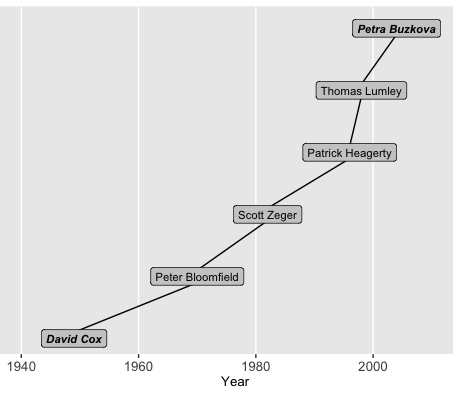
\includegraphics[width=0.7\textwidth]{pathCB}
    \end{framed}
    \caption{The shortest path between Sir David Cox and one of his fifth generation "descendants", Petra Buzkova.}
    \label{fig:pathCB}
\end{figure}

This code results in Figure \ref{fig:pathCB}. We see that the shortest path between Sir David Cox and Petra Buzkova is strictly composed of five unidirectional "parent-child" relationships that span about 55 years. We see that the time difference between when an advisor and student earned their degrees is not consistent across this path: The three statisticians who earned their degrees earliest in this path span more than 30 years in degree acquisition, whereas the three statisticians who earned their degrees later in this path only span less than ten years in degree acquisition.

We also notice in Figure \ref{fig:pathCB} that Sir David Cox received his statistics degree in about 1950, and Petra Buzkova received her statistics degree in about 2005. This genealogy only contains historical information about obtained degrees, and does not project into the future. Hence, we can be assured that Petra Buzkova is one of the younger individuals in the dataset, at least in the sense that the youngest individual could only have received his or her degree ten years after Petra Buzkova. However, we cannot be assured that Sir David Cox is one of the oldest individuals in the dataset. As such, it would be informative to superimpose this path of interest onto the entire dataset, using the \code{plotPathOnAll()} function of the \pkg{ggenealogy} package, as we did for the soybean genealogy in Figures \ref{fig:plotTNBin3} and \ref{fig:plotTNBin6}.

We can achieve this using the below code. After trial and error, we use a \code{binVector} of size 200, and append \pkg{ggplot2} syntax to define suitable x-axis limits. The output of this process is illustrated in Figure \ref{fig:plotCBText}.

\mybox{
\texttt{R> plotPathOnAll(pathCB, statGeneal, statIG, binVector = 1:200) + ggplot2::theme(axis.text = ggplot2::element\_text(size = 8), axis.title = ggplot2::element\_text(size = 8)) + ggplot2::scale\_x\_continuous(expand = c(.1, .2))}
}

\begin{figure}[H]
    \begin{framed}
    \centering
    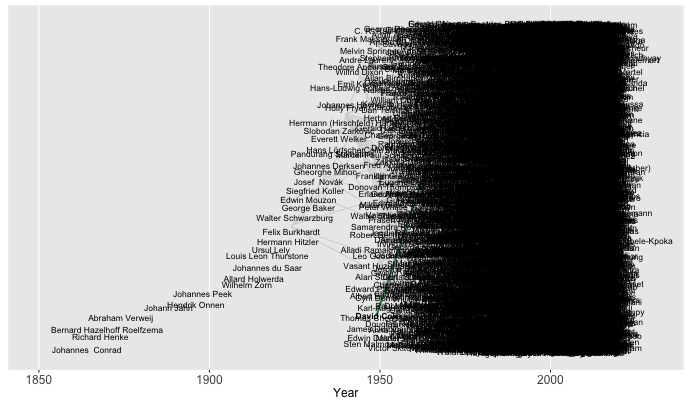
\includegraphics[width=\textwidth]{plotCBText}
    \end{framed}
    \caption{The shortest path between Sir David Cox and Petra Buzkova, superimposed over the data structure, using a bin size of 200.}
    \label{fig:plotCBText}
\end{figure}

We see from the resulting Figure \ref{fig:plotCBText} that almost all text labels for individuals who received their graduate-level statistics degrees between 1950 and 2015 are undecipherable. We also see that the year Sir David Cox acquired his statistics degree is somewhere in the later half of the variable year for this dataset, as the oldest dates for acquisition of statistics degrees in this dataset occur around 1860. However, the number of individuals who are documented as receiving their statistics degrees between 1860 and 1950 are few enough so that their text labels are somewhat readable.

The text labels are so numerous in Figure \ref{fig:plotCBText} that simply trying different values for the input parameter \code{binVector} will not solve the text overlapping problem. Instead, one approach we can try is to reconstruct the plot using the same \pkg{ggenealogy} function \code{plotPathOnAll()}, only now specifying variables to render the size (2.5) and color (default of black) of the text for nodes that are on the path of interest to be more noticeable than the size (0.5) and color (dark gray) of the text for nodes thare not on the path of interest. Moreover, we can make the edges that are not on the path of interest to be represented in a less noticeable color (light gray) than the edges that are on the path of interest (default of dark green). The variable names and options for these aesthetics is further detailed in the help manual of the function. We provide one example code that alters the defaults of the text color and sizes of nodes and edges below, which results in Figure \ref{fig:plotCBNoText}.

\mybox{
\texttt{R> plotPathOnAll(pathCB, statGeneal, statIG, binVector = 1:200, nodeSize = .5, pathNodeSize = 2.5, nodeCol = "darkgray", edgeCol = "lightgray") + ggplot2::theme(axis.text = ggplot2::element\_text(size = 8), axis.title = ggplot2::element\_text(size = 8)) + ggplot2::scale\_x\_continuous(expand = c(.1, .2))}
}

\begin{figure}[H]
    \begin{framed}
    \centering
    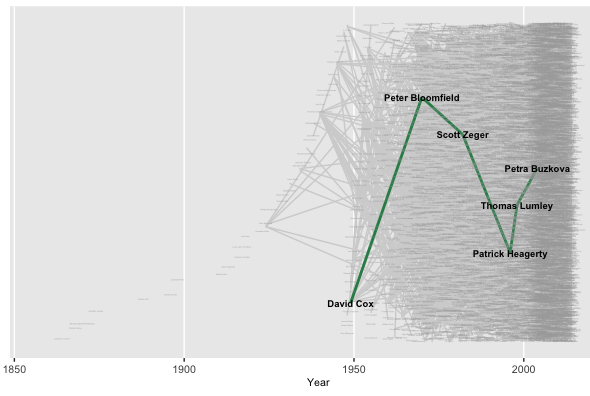
\includegraphics[width=\textwidth]{plotCBNoText}
    \end{framed}
    \caption{The shortest path between Sir David Cox and Petra Buzkova, superimposed over the data structure, using a bin size of 200. Individuals on the shortest path are labeled in large and black text and connected by dark green edges; all other individuals are labeled in small and gray text and connected by light gray edges.}
    \label{fig:plotCBNoText}
\end{figure}

In Figure \ref{fig:plotCBNoText}, we can now see each individual on the path of interest, and how their values for the variable year are overlaid on the entire genealogy structure. We can also more clearly see that, even though only ten years span between the youngest individual in the genealogy and Petra Buzkova, there are many individuals in that last decade. Indeed, the decade from 2005 to 2015 appears to be the densest in this dataset in terms of acquisition of statistics degrees.

\subsection{Interactive visualization of genealogical structure}

We could still improve upon Figure \ref{fig:plotCBNoText}. Even though we may be primarily interested in understanding how the path of interest is overlaid across the entire genealogical structure, we could, upon viewing the entire structure, also develop an interest in nodes that are not on the path of interest but are revealed to stand out among the rest of the genealogical structure. For instance, in Figure \ref{fig:plotCBNoText}, it may be of interest for us to determine the names of the few individuals who obtained their statistics degrees before 1900. Fortunately, within the \code{plotPathOnAll()} function, there is a variable \code{animate} that we can set to a value of TRUE to create an interactive version of the figure that allows us to hover over individual illegible labels and immediately receive their labels in a readable format. A short video demonstration of these interactive features can be viewed upon clicking on Figure \ref{fig:plotAnimate}.

\mybox{
\texttt{R> plotPathOnAll(pathCB, statGeneal, statIG, binVector = 1:200, nodeSize = .5, pathNodeSize = 2.5, nodeCol = "darkgray", edgeCol = "lightgray", animate = TRUE)}
}

\begin{figure}[H]
    \begin{framed}
    \centering
    \includemedia[width=1.0\textwidth, addresource=animateGen.mov, deactivate=onclick, flashvars={source=animateGen.mov}]{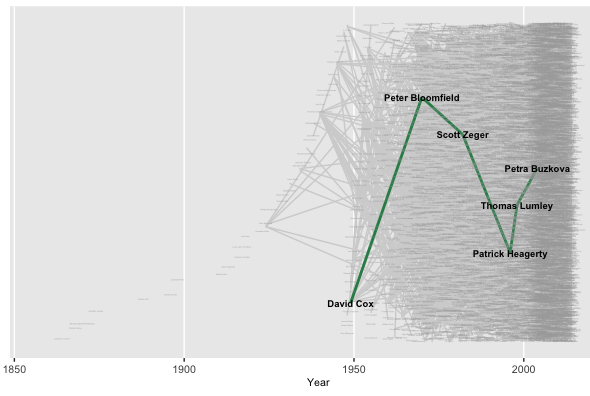
\includegraphics{./plotCBNoText.png}}{VPlayer.swf}
    \end{framed}
    \caption{Upon clicking on this figure twice, a short video demonstrating the animation features for this function can be viewed. Please note that to properly view this video, the PDF version of this paper must be opened in Adobe Acrobat Reader DC (Version >=9), which can be downloaded free of charge.}
    \label{fig:plotAnimate}
\end{figure}

\section{Future Avenues}

We have several avenues we could pursue to expand upon this work:

\begin{enumerate}
\item \textbf{Incorporation of the Shiny application}: The reactive programming could save users of \pkg{ggenealogy} the time of using command line for each change of input as well as the inefficiency of rerunning code. It could also enhance the interactivity. A Shiny application that uses certain \pkg{ggenealogy} functionality is already available for users who wish to explore the soybean genealogy; the data can be viewed at \url{http://shiny.soybase.org/CNV/}.

\item \textbf{Expanding on variable types}: We could incorporate plotting tools that examine not only quantitative variables (such as our example variable of "year"), but also categorical variables associated with individuals in datasets.

\item \textbf{Further eliminate text overlap}: The \pkg{ggenealogy} visualization tool \code{plotPathOnAll()} is suitable as a data exploration tool, but not always as a publication tool. This is because we still see textual overlap in datasets that are small enough to - in theory - be represented with all labels in a readable format (see Figure \ref{fig:plotTNBin6}). As such, we plan to add a feature to the package that allows users to manually fine-tune automated plots. For example, after comparing several bin sizes on the soybean genealogy, we determined that the bin size of 6 produced the minimal textual overlap, as is seen in Figure \ref{fig:plotTNBin6}. If we could subsequently fine-tune the vertical positions of the small fraction of text labels that remained overlapped after the automated \pkg{ggenealogy} function, then we could potentially remove all overlaps, and the plot could be used in presentations and publications.

\item \textbf{Test on additional datasets}: We look forward to testing the \pkg{ggenealogy} package on additional genealogical data sets. Exploring several datasets with the software will allow us to fix remaining bugs, and provide us further insight into how to make our tools available for a wide range of data input formats. 
\end{enumerate}

\section{Conclusions}

The \pkg{ggenealogy} package offers various plotting tools that can assist those studying genealogical lineages in the data exploration phases, as well as in preparing publication-suitable images. As each plot comes with its pros and cons, we recommended for users to explore several visualization tools. If users are simultaneously using similar packages, we in particular recommend using the \code{plotAncDes()} function. This plot allows users to view generation counts of a variety of interest in a manner that is not as readily available in similar software packages.

\section{Acknowledgments}

This project was an effort between Susan VanderPlas, Dianne Cook, Michelle A. Graham, and myself. Together, we  thank Drs. James E. Specht and Randy C. Shoemaker for helpful discussions of soybean genealogy. In addition, we are grateful for the financial support from the United Soybean Board (Project 1204), The North Central Soybean Research Program, the NSF Plant Genome Research Program (award number 0820642), and the USDA-ARS CRIS Project 3625-21220-005-00D. The USDA is an equal opportunity provider and employer. Mention of trade names or commercial products in this article is solely for the purpose of providing specific information and does not imply recommendation or endorsement by the U.S. Department of Agriculture.










%%%%%%%%%%%%%%%%%%%%%%%%%%%%%%%%%%%%%% CHAPTER %%%%%%%%%%%%%%%%%%%%%%%%%%%%%%%%%%%%%% 
%%%%%%%%%%%%%%%%%%%%%%%%%%%%%%%%%%%%%%%%%%%%%%%%%%%%%%%%%%%%%%%%%%%%%%%%%%%%%%%%%%%%%

\chapter{Visualization methods for clustering analysis of RNA-sequencing data}
\label{sec:clustering}

\section{Introduction}

In plants, iron is a necessary micronutrient for photosynthesis, respiration, and other metabolic processes. Iron uptake from the soil, iron transportation, and iron storage are all tightly regulated in plants to maintain homeostatic balance. A surplus of iron can cause cellular damage, but a deficiency in iron can cause Iron Deficiency Chlorosis (IDC), which causes yellowing of leaves and eventually total yield loss (\citealt{soy1}). While it is a global problem, IDC is particularly problematic where the majority of soybeans in the United States are grown in the calcareous soils of the Midwesten United States (\citealt{soy3}). One recommended strategy for controlling IDC is to develop IDC-resistant soybean lines. However, IDC-resistant soybean lines do not have as high of a yield as IDC-susceptible lines in iron-sufficent conditions. As a result, developing IDC-resistant soybean lines with high yield in multiple soil types is ideal.

In recent years, identification of soybean genes that are differentially expressed during iron stress and recovery have been determined with the use of microarray analyses, RNA-sequencing, and virus-induced gene silencing (VIGS) (\citealt{soy11}, \citealt{soy12}, \citealt{soy13}, \citealt{soy14}, and \citealt{soy15}). However, much remains elusive about early signaling processes in iron-efficient stress responses. In the early 1970s, two soybean cultivars (Clark and Isoclark) with similar genotypes but different responses to iron stress were developed (\citealt{soy10}). Clark is an iron-efficient line that is resistant to IDC development in iron-poor conditions. In contrast, Isoclark is not an iron-efficient line and is susceptible to IDC development in iron-poor conditions.

\section{Example Dataset}

The dataset comes from an RNA-sequencing study conducted to identify early signaling responses between roots and leaves in iron stress conditions in the iron-efficient soybean line Clark. To this end, a total of 36 samples of the cultivar Clark were exposed to iron-deficient and iron-sufficent soil conditions for 30 minutes, 60 minutes, and 120 minutes. A more detailed and similar methodology can be found in (\citealt{adSoy}).

Genes will be clustered into groups that showed similar changes in read counts across iron condition, time point, and/or biological derivative (roots or leaves). The resulting clusters could help us identify what genes are responsible for how, when, and where soybeans respond to iron-deficient environments. Our dataset of interest has a structure as follows:

\begin{itemize}
  \item Count table for 56,044 genes in 18 samples of soybean leaves
  \begin{itemize}
    \item 30 minutes after iron-rich soil (3 replicates)
    \item 60 minutes after iron-rich soil (3 replicates)
    \item 120 minutes after iron-rich soil (3 replicates)
    \item 30 minutes after iron-deficient soil (3 replicates)
    \item 60 minutes after iron-deficient soil (3 replicates)
    \item 120 minutes after iron-deficient soil (3 replicates)
  \end{itemize}
  \item Count table for 56,044 genes in 18 samples of soybean roots
    \begin{itemize}
    \item 30 minutes after iron-rich soil (3 replicates)
    \item 60 minutes after iron-rich soil (3 replicates)
    \item 120 minutes after iron-rich soil (3 replicates)
    \item 30 minutes after iron-deficient soil (3 replicates)
    \item 60 minutes after iron-deficient soil (3 replicates)
    \item 120 minutes after iron-deficient soil (3 replicates)
  \end{itemize}
\end{itemize}

\section{Pre-processing}

Exploratory data analysis was performed to better understand the data, to serve as a quality check, and to prepare for pre-processing analysis. It consisted of three main approaches:

\begin{itemize}

\item \textbf{Normalization}: Only a small fraction of the 56,044 genes should demonstrate read count changes of interest. We had to first determine what type of normalization to perform in order to standardize the gene read count distribution across the samples, so that the vast majority of genes do not artificially appear important.

\item \textbf{Remove Genes with Low-Counts and Low-Variability}: We removed the bottom quartile of genes with low mean read counts, and we also removed the bottom quartile of genes with low standard deviaton in read counts.

\item \textbf{Quality and Label Checking}: We check the quality of our data by analyzing pairwise scatterplot matrices of intra- versus inter- replicates and MDS plots. With these visual tools, we would expect high-quality genes to show replicates with consistency (low variability) in counts.

\end{itemize}

It would be difficult (if not impossible) to determine how consistent the samples are with a parallel coordinate plot. Instead, we began by examining a side-by-side boxplot of all 36 samples. From this plot, we believe the data will require intense normalization (see Figure \ref{fig:needNorm}).

\begin{figure}[H]
    \begin{framed}
    \centering
    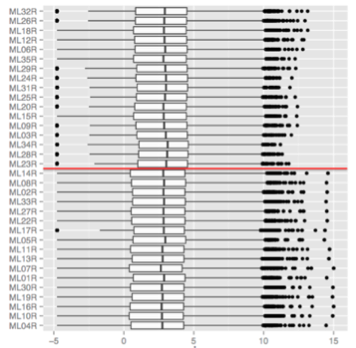
\includegraphics[width=\textwidth]{needNorm}
    \end{framed}
    \caption{Boxplot of the all leaves and roots samples before any normalization method. Since we only expect a handful of genes to show differential expression, we expect the samples to be mostly similar. However, we see here that there is a systematic error between the leaves and roots. Namely, the roots (above the horizontal blue line) have a larger median number of counts, and also tend to have more low-valued outliers. There is even variation within roots and leaves (although to a much less extent than between the two groups). This all means that we need to heavily normalize this data.}
    \label{fig:needNorm}
\end{figure}

Next, we created an MDS plot to better understand the quality of the data (\citealt{limma}). Based on this MDS plot, we determine that the six samples of leaves from 120 minutes appear to be of the best quality from this dataset (see Figure \ref{fig:mdsGroups}).

\begin{figure}[H]
    \begin{framed}
    \centering
    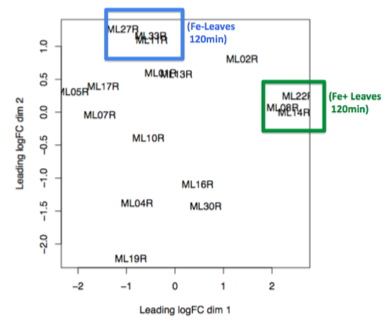
\includegraphics[width=\textwidth]{mdsGroups}
    \end{framed}
    \caption{MDS plot of the six samples of leaves from 120 minutes. If the data is high-quality, then each of the three replicates should be separated very only a little distance, and inter-replicates should be separated by a further distance. We see that the 120-minute leaves in iron-deficient conditions (8, 14, and 22) and iron-sufficient conditions (11, 27, and 33) are possibly high-quality data. However, most of the rest of the MDS plot is messy, indicating that the rest of the leaves data is probably of poor-quality.}
    \label{fig:mdsGroups}
\end{figure}

\section{Highest quality replicates (Leaves at 120 minutes)}

Because these visual tools made us believe that the leaves from 120 minutes were of the highest quality, we subsetted the data to only consider these six samples for the time being. First, we converted the read counts to counts per million (cpm), because raw counts  do not account for differences in library sizes between samples. We then placed the cpm count values on a logarithmic scale.

We then prepared to examine this subset of the data by heavily filtering it. In general, genes should be discarded if they have zero probability of being expressed in all the samples for any of the treatments (\citealt{edger}). We first applied this rule of thumb, but then we continued to filter more extensively. Namely, we calculated the mean and standard deviation read count for the six samples, and removed the genes with the lowest quartile of mean read count, as well as the genes with the lowest quartile of standard deviation read count across the six samples. Finally, we removed genes that contained negative residuals from a Loess fit, as these genes were unlikely to be of interest, having low mean and standard deviation read counts (see Figure \ref{fig:loessL120}).

\begin{figure}[H]
    \begin{framed}
    \centering
    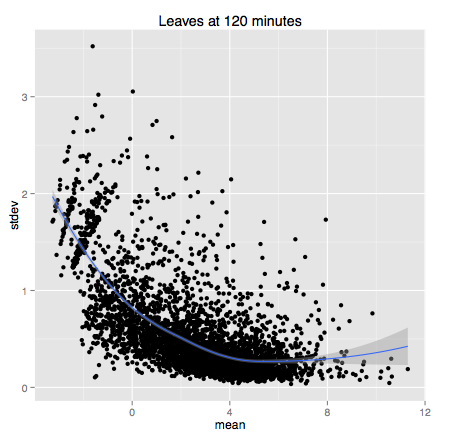
\includegraphics[width=\textwidth]{loessL120}
    \end{framed}
    \caption{Plot of all genes with the standard deviation versus mean read count of the 6 leaf samples at 120 minutes. Any genes below the Loess fit (shown in blue) were removed for having a low standard deviation and mean read count across the samples.}
    \label{fig:loessL120}
\end{figure}

After filtering and normalizing on the six samples of interest (leaves at 120 minutes), we then checked the quality again by creating a scatterplot matrix, which confirmed that this subset of the data had potential for trustworthy analysis (see Figure \ref{fig:L120scatter}).

\begin{figure}[H]
    \begin{framed}
    \centering
    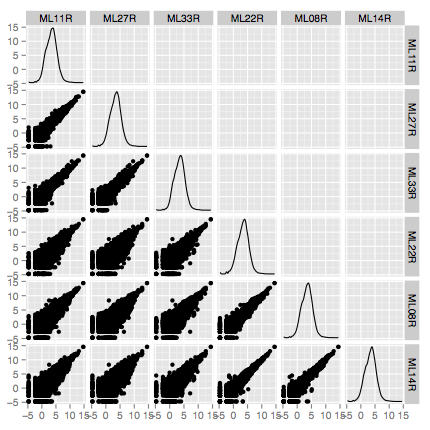
\includegraphics[width=\textwidth]{L120scatter}
    \end{framed}
    \caption{Scatterplot matrix of the six samples of leaves from 120 minutes, where each individual scatterplot matrix compares two of the six samples. If the 120-minute leaves samples are high quality, then we would expect replicates to have read counts centered on the diagonal x=y line, and non-relicates to deviate somewhat from the diagonal x=y line. Indeed, this is what we see, as the bottom-left nine plots (non-replicates) appear much thicker around the x=y line than the other plots (replicates).}
    \label{fig:L120scatter}
\end{figure}

Now that the data of the leaf samples at 120 minutes has been properly pre-processed, we began the clustering analysis by producing a dendogram. We used Euclidean distance (which is acceptable as we have standardized the data) and hiearchical clustering with Wards linkage.

\begin{figure}[H]
    \begin{framed}
    \centering
    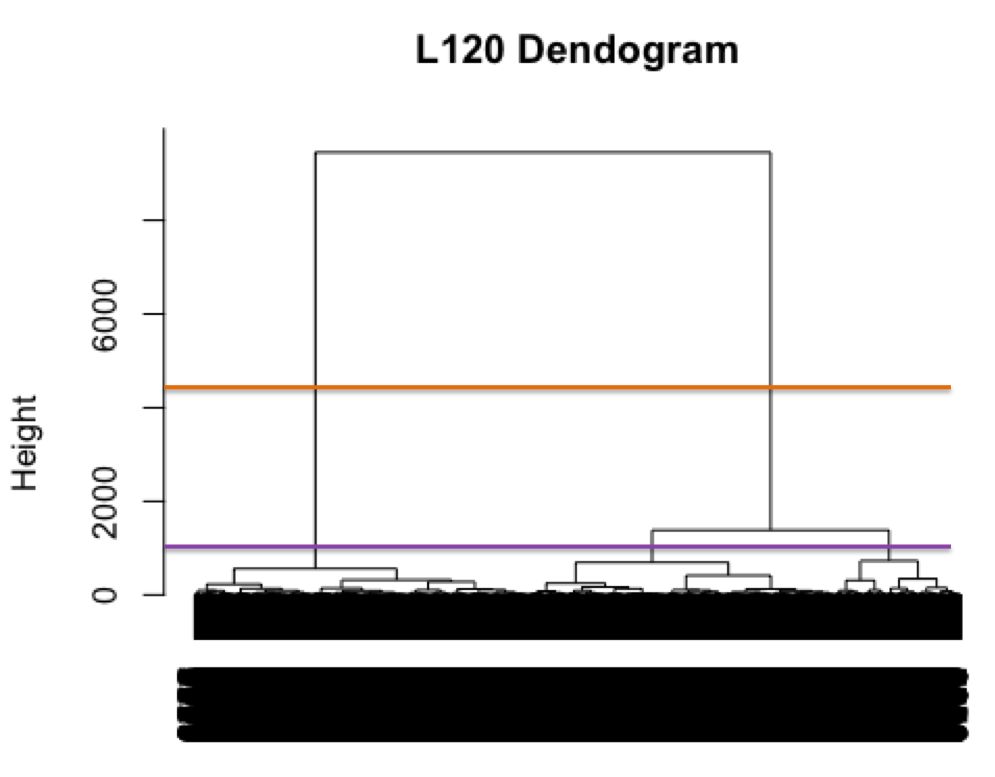
\includegraphics[width=\textwidth]{dendL120}
    \end{framed}
    \caption{The dendogram of the 6 leaf samples at 120 minutes. We see that there may be two main clusters (designated by the orange cut), and possibly a third smaller cluster (designated by the purple cut).}
    \label{fig:dendL120}
\end{figure}

\subsection{Two clusters}

We first examined how the data separates into the two main clusters indicated in the dendogram of Figure \ref{fig:dendL120}. To do so, we cut the hierarchical tree, and then constructed a parallel coordinate plot of the resulting two clusters, along with the previously-filtered data (see Figure \ref{fig:pcp2L120}).

\begin{figure}[H]
    \begin{framed}
    \centering
    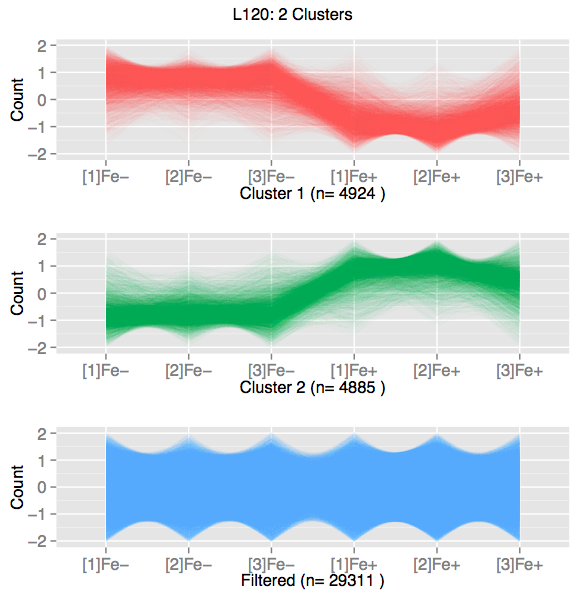
\includegraphics[width=\textwidth]{pcp2L120}
    \end{framed}
    \caption{Parallel coordinate plot of the two clusters and filtered data, where each line represents the standardized read count for a given gene across the 6 leaf samples from 120 minutes. As the dendogram in Figure \ref{fig:dendL120} suggested 2 clusters for the 6 samples, we applied a k-means clustering algorithm with a cluster size of 2, resulting in the pink cluster and green cluster above. We see that the pink cluster contains genes higher in the Fe- samples, whereas the green cluster contains genes higher in the Fe+ samples. Both clusters look relatively clean (their repetitions are horizontal). In blue, we see the genes that were filtered, in the process previously described. This is relatively flat across all six samples, as we would expect.}
    \label{fig:pcp2L120}
\end{figure}

Additionally, we can examine what these two clusters look like in a scatterplot (shown in Figure \ref{fig:scatterL120}).

\begin{figure}[H]
    \begin{framed}
    \centering
    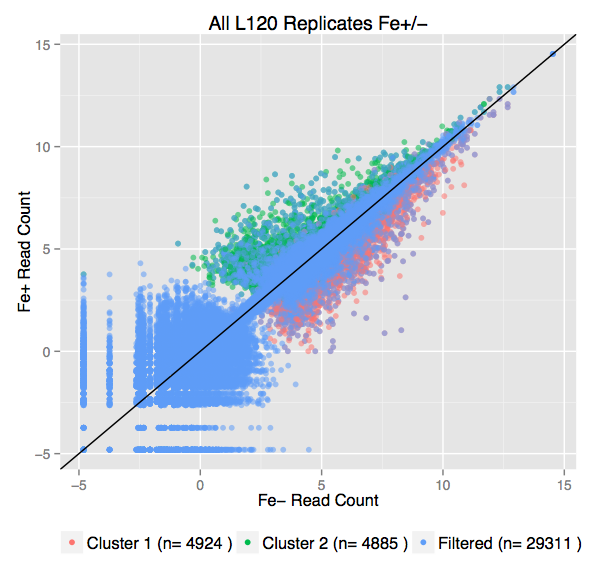
\includegraphics[width=\textwidth]{scatterL120}
    \end{framed}
    \caption{A scatterplot, where each dot represents the raw read counts from a gene in iron-deficient (x-axis) and iron-sufficient (y-axis) conditions from the leaf samples at 120 minutes. The pink and green colors represent the two clusters created when a k-means algorithm of cluster size 2 was applied, and the blue color represents the data filtered out as described at the beginning of the paper. The image is consistent with Figure \ref{fig:pcp2L120}, and the pink cluster appears to have lower Fe+ read counts, while the green cluster appears to have lower Fe- read counts. The blue cluster is, as expected, more closely along the x-y axis.}
    \label{fig:scatterL120}
\end{figure}

\subsection{Three clusters}

We next look at how the data separates into the three main clusters indicated in the dendogram of Figure \ref{fig:dendL120}. We perform the appropriate heirarchical cut on the data, and then construct a parallel coordinate plot of the resulting three clusters, along with the previously-filtered data, see Figure \ref{fig:pcp3L120}.

\begin{figure}[H]
  \begin{framed}
  \centering
  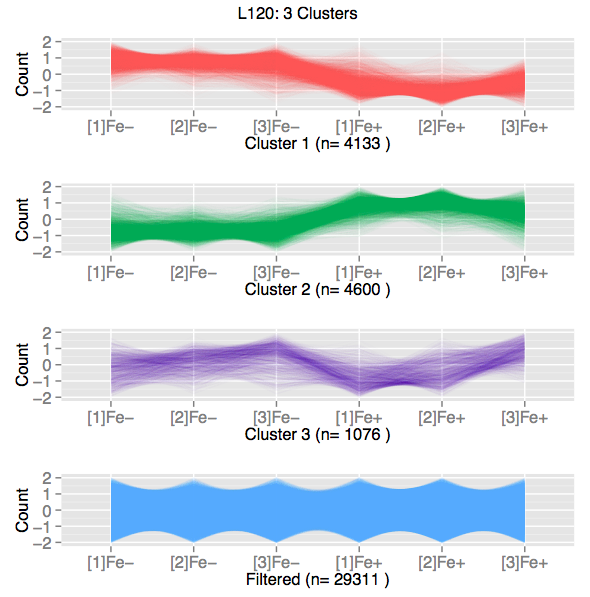
\includegraphics[width=\textwidth]{pcp3L120}
  \end{framed}
  \caption{Parallel coordinate plot of the three clusters and filtered data, where each line represents the standardized read count for a given gene across the 6 leaf samples from 120 minutes. As the dendogram in Figure \ref{fig:dendL120} suggested 3 clusters for the 6 samples, we cut the data accordingly, resulting in the pink, green, and purple clusters above. We see that the pink cluster contains genes higher in the Fe- samples, whereas the green cluster contains genes higher in the Fe+ samples. Both clusters look relatively clean (their repetitions are horizontal). In blue, we see the genes that were filtered, in the process previously described. This is relatively flat across all six samples, as we would expect. All of this is similar to what we saw in Figure \ref{fig:pcp2L120}, where we examined 2 clusters. What is new is the purple cluster, which appears similar to the pink cluster (in that it is lower in the Fe+ read counts), except for the third repetition, which seems inconsisent. This purple cluster may represent low-quality genes.}
  \label{fig:pcp3L120}
\end{figure}

We can again view this data in a scatterplot matrix format (see Figure \ref{fig:3scatterL120}).

\begin{figure}[H]
  \begin{framed}
  \centering
  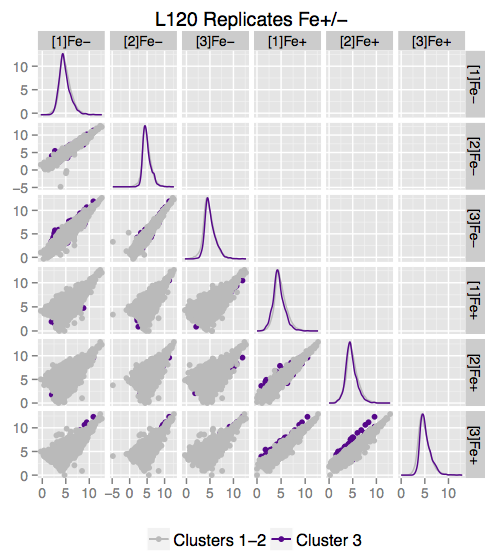
\includegraphics[width=\textwidth]{3scatterL120}
  \end{framed}
  \caption{Scatterplot matrix of the three clusters from the leaves in 120 minutes, where the purple cluster that looked problematic in the parallel coordinate plot in Figure \ref{fig:pcp3L120} is also colored purple here, and all other data is colored grey. We see that our suspicions from the parallel coordinate plot that the purple cluster was poor-quality have been corroborated here; the third repetition from the Fe+ sample appears to be the cause of the streaks seen most prominently in the bottom-right scatterplot.}
  \label{fig:3scatterL120}
\end{figure}

Based on our parallel coordinate plot in Figure \ref{fig:pcp3L120} and our scatterplot matrix in Figure \ref{fig:3scatterL120}, when this data is clustered into three groups, one of these clusters (the purple cluster) may be of poor quality (inconsistency between replicates). At this point, it may be helpful to examine some of the 1076 genes in this third cluster individually. In Figures \ref{fig:indSBGenes1} and \ref{fig:indSBGenes2}, we show a more detailed (genewise) view of a random sample of 24 genes from this third cluster.

\begin{figure}[H]
  \centering
  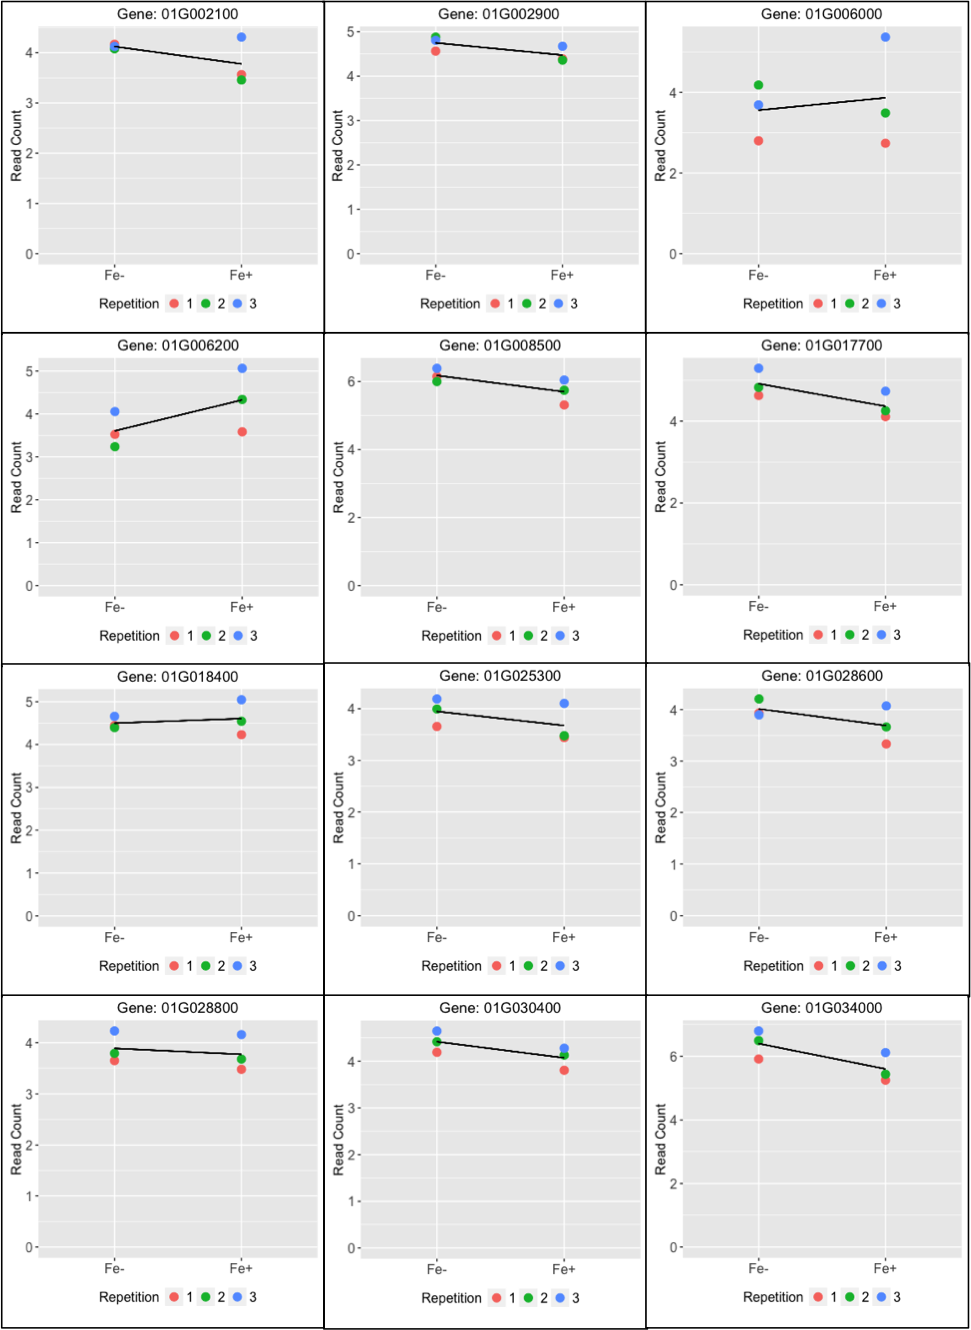
\includegraphics[width=\textwidth]{indSBGenes1}
  \caption{One random sample of 12 genes from the third problematic-looking purple cluster. We see that many of these genes confirm the patterns we saw in the third cluster in Figures \ref{fig:pcp3L120} and \ref{fig:3scatterL120}. Namely, they tended to show smaller read counts in the Fe+ condition than the Fe- condition, except for a disconcerningly large read count for the third replicate of the Fe- condition.}
  \label{fig:indSBGenes1}
\end{figure}

\begin{figure}[H]
  \centering
  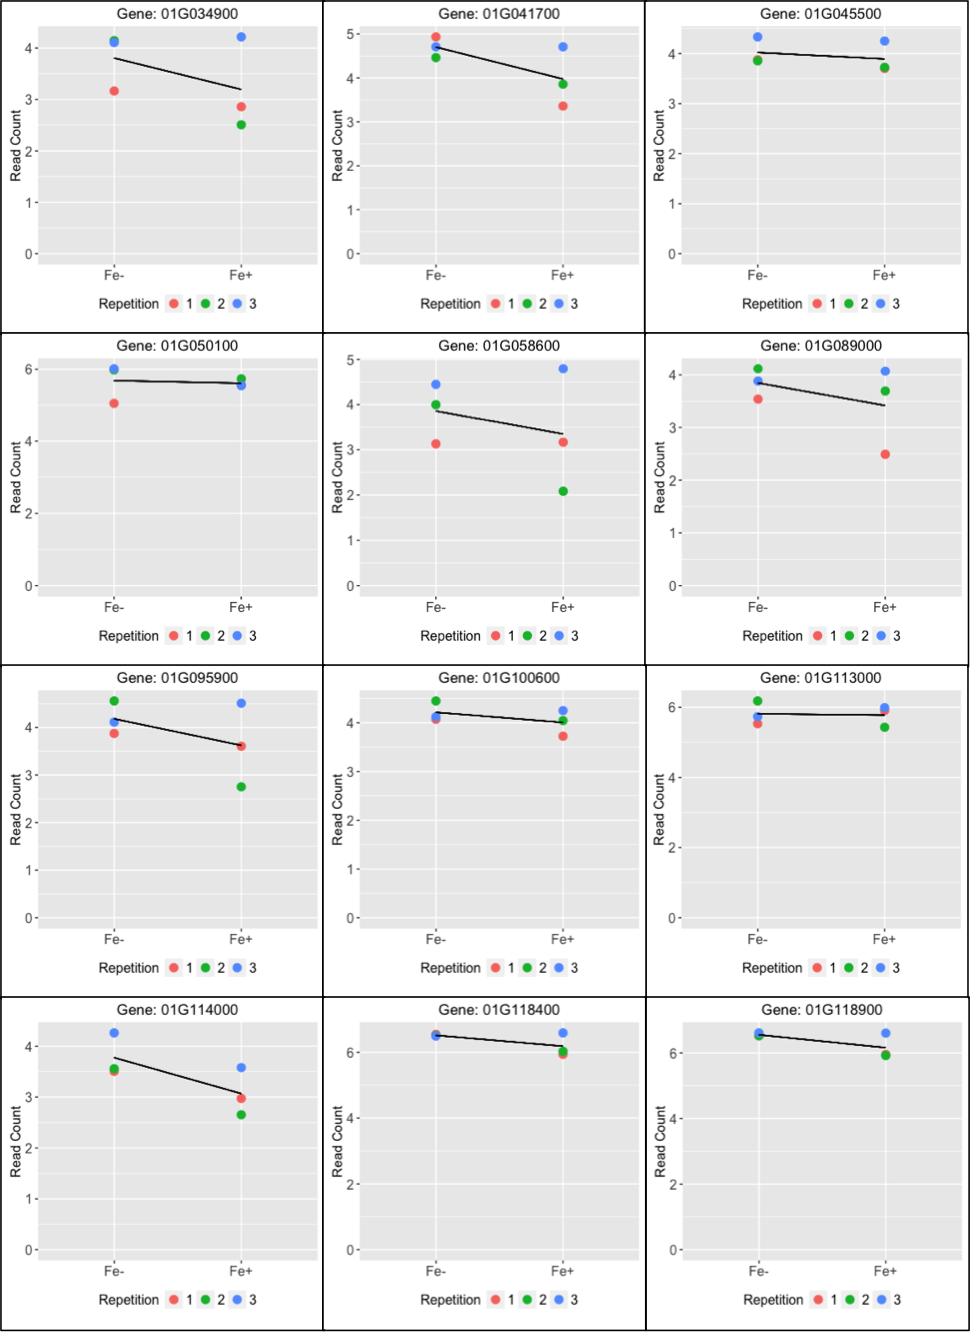
\includegraphics[width=\textwidth]{indSBGenes2}
  \caption{A second random sample of 12 genes from the third problematic-looking purple cluster. We see that many of these genes confirm the patterns we saw in the third cluster in Figures \ref{fig:pcp3L120} and \ref{fig:3scatterL120}. Namely, they tended to show smaller read counts in the Fe+ condition than the Fe- condition, except for a disconcerningly large read counts for the third replicates of the Fe- condition.}
  \label{fig:indSBGenes2}
\end{figure}

\subsection{Many clusters}
\label{sec:manyClusters}

By going from two clusters to three clusters, it seems that we were able to discard 1076 genes, many of which would not be of interest to us as they demonstrate poor consistency in the third replication of the Fe- condition. However, not all (or even a majority) of the genes from this cluster follow this pattern of poor consistency in the third replication of the Fe-condition. Moreover, we are still left with 8733 unfiltered genes (4133 genes from the first cluster and 4600 genes from the second cluster), which would be too many genes to make any coherent biological implications.  

For these reasons, we may now wish to apply increasingly larger cluster cuts so that we can continue to discard genes by grouping them into clusters that indicate poor quality (inconsistent replications) or indifference to the treatment of interest (consistent values between treatment groups). At the same time, this process will refine our set of genes that remain undiscarded, by sifting through the clusters that indicate high quality (consistent replications) and response to treatments (inconsistent values between treatment groups) to remove the genes that should not be present in those groups in the first place.

We have created a script for users that allows them to designate the maximum cluster size they wish to cut. It then outputs into a folder for them the following items:

\begin{itemize}

\item One PDF file that contains the parallel coordinate plot for each cluster cut size between two (just like Figure \ref{fig:pcp3L120}) and the maxmimum cluster size of their choice.

\item A JPG file of the parallel coordinate plot for each cluster in each cluster cut size (between two and the maximum cluster size of their choice). This would result in $2+3+4+5+6+7+8+9+10+11+12+13+14+15=199$ JPG files.

\item A TXT file listing the names of the genes present for each cluster in each cluster cut size (between two and the maximum cluster size of their choice). This would result in $2+3+4+5+6+7+8+9+10+11+12+13+14+15=199$ TXT files.

\end{itemize}

This PDF file that is output from this script allows users to obtain a quick overview of the cluster analysis, specifically what clusters of genes look like across different cluster cut sizes (between two and the maximum cluster size of their choice). At the same time, the JPG files allow users to see the more detailed images of what an individual cluster of interest looks like, and the TXT files allows users to obtain detailed information about the gene names of an individual cluster of interest.

For example, we conducted an analysis using a maximum cluster size of 15. In the output PDF file, we could see what the 14 parallel coordinate plots looked like using cluster sizes of 2 and 15 inclusively. This PDF file could allow users to obtain a sense of what might be an appropriate cutoff for cluster size. The last parallel coordinate plot for the cluster of size 15 is shown in Figure \ref{fig:L120_15}.

\begin{figure}[H]
  \begin{framed}
  \centering
  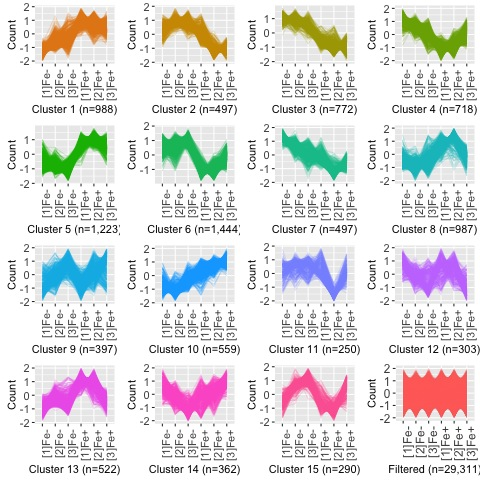
\includegraphics[width=\textwidth]{L120_15}
  \end{framed}
  \caption{Parallel coordinate plots for the resulting 15 clusters (and the filtered cluster) when the user defines a maximum cluster size of 15. Just like we created the purple cluster with the suspiciously poor-quality third replication of the Fe+ treatment, we have now created many additional clusters that may not be of interest to us due to poor quality: For instance, Cluster 11 contains a group of 250 genes that may have suspiciously low read counts in the second replication of the Fe+ group, and Cluster 2 contains a group of 497 genes that may have suspiciously high read counts in the first replication of the Fe+ group. We have also created clusers that may not be of interest to us due to lack of response to treatements: For instance, Clusters 3, 7, 10, and 14 all show a relatively flat line across the six samples, and the 2190 genes contained between these four clusters may be considered for removal.}
  \label{fig:L120_15}
\end{figure}

Many of these 15 clusters are not of interest to us due to poor quality between replicates or lack of response to treatments. From Figure \ref{fig:L120_15}, it seems that perhaps the clusters that contain the genes of interest may be Cluster 5 (good replication quality and more read counts in Fe+) and Cluster 6 (good replication quality and more read counts in Fe-).

In the output directory, we would have the TXT files that list the 1223 genes that belong to Cluster 5 and the 1444 genes that belong to Cluster 6. We would also have the individual JPG files for these two clusters that could allow us to view their parallel coordinate plots in greater detail:

\begin{figure}[H]
  \begin{framed}
  \centering
  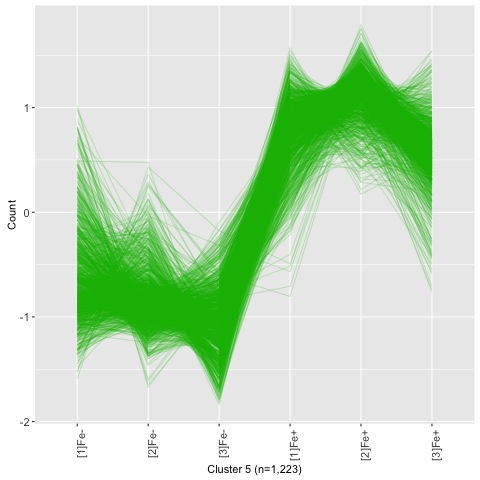
\includegraphics[width=\textwidth]{L120_15_5}
  \end{framed}
  \caption{Parallel coordinate plot with a more detailed view of the 1223 genes in Cluster 5 when a cluster cut size of 15 was applied. This cluster appears to belong to genes that were more highly expressed in Fe- conditions than Fe+ conditions.}
  \label{fig:L120_15_5}
\end{figure}

\begin{figure}[H]
  \begin{framed}
  \centering
  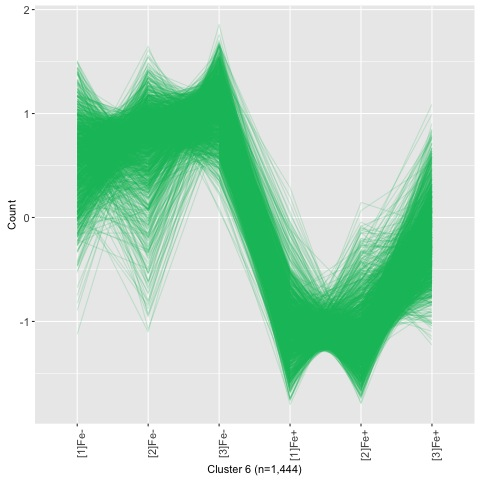
\includegraphics[width=\textwidth]{L120_15_6}
  \end{framed}
  \caption{Parallel coordinate plot with a more detailed view of the 1444 genes in Cluster 6 when a cluster cut size of 15 was applied. This cluster appears to belong to genes that were more highly expressed in Fe+ conditions than Fe- conditions. However, it appears that some of the problem with the poor-quality replicate that we saw in the purple cluster of Figure \ref{fig:pcp3L120} is still present.}
  \label{fig:L120_15_6}
\end{figure}

Overall, increasing the cluster cut size from 2 to 15 reduced the total number of genes in our two clusters of interest from 9809 to 2667 genes. This may still be too large of a number of genes to work with and the quality of the two clusters - even at a cluster cut size of 15 - could still be improved with an even larger cut size.

\section{Future Avenues}

We have several avenues we could pursue to expand upon this work:

\begin{enumerate}
\item \textbf{Render the parallel coordinate plots interactive}: We showed in Section \ref{sec:manyClusters} that we have developed a script that allows users to quickly view the details of clusters from different cluster cut sizes. The ideas behind the speed and usefulness of this script would be enhanced if we incorporated interactive capabilities. For instance, there could be an interactive function that allows users to zoom in on a cluster of interest, select individual genes (lines), and remove genes from the cluster manually if they do not appear to be of interest.

\item \textbf{Adapt parallel coordinate plots to large datasets}: We still face space (overplotting) and time (computational speed) constraints. As such, our goal is to adapt the parallel coordinate plot to large amounts of data.

\item \textbf{Develop guidelines for scatterplot matrices}: Developing guidelines for scatterplot matrix interpretations would be useful. We want to develop a recommended threshold to dictate whether or not the variability between the replications is appropriate. This could be particularly important as even just a few genes distanced from the expected x=y line could be misleading if the dataset is large.

\item \textbf{Adapt scatterplot matrices to large datasets}: We still face space (overplotting) and time (computational speed) constraints. As such, our goal is to adapt the scatterplot to large amounts of data.

\item \textbf{Render the individual gene plots interactive}: As we demonstrated in Figures \ref{fig:indSBGenes1} and \ref{fig:indSBGenes1}, it proves useful to also examine the genes from clusters of interest at their individual levels. It would be even more helpful to have an interactive function so that users can flip through these images rapidly, and possibly remove genes from the cluster manually if they do not appear to be of interest.

\end{enumerate}

\section{Conclusions}

The preliminary results from our visualization methods of clustering analysis of RNA-sequencing data are promising: We conclude that cluster analysis provided us with clusters of genes that may have marked different expression across time, iron environment, and biological derivative (leaf versus root), and that we could use visual tools to better understand the results. Our approach could still be greatly improved; we have obtained a better specified and more complete list of future avenue directions with our preliminary results. 

\section{Acknowledgments}

\textbf{\textcolor{Red}{What should I put here?}}






%%%%%%%%%%%%%%%%%%%%%%%%%%%%%%%%%%%%%% CHAPTER %%%%%%%%%%%%%%%%%%%%%%%%%%%%%%%%%%%%%% 
%%%%%%%%%%%%%%%%%%%%%%%%%%%%%%%%%%%%%%%%%%%%%%%%%%%%%%%%%%%%%%%%%%%%%%%%%%%%%%%%%%%%%

\chapter{Visualization methods for significance testing of RNA-sequencing data}
\label{sec:sigtest}

\section{Introduction}

Phenotypic plasticity is an adaptive tool in which a given genotype has the ability to produce more than one phenotype when exposed to different biotic and abiotic environmental factors (\citealt{pw4}). Reproductive castes in social Hymenoptera (wasps, ants, and bees) provide one of the most-researched models of insect phenotypic plasticity (\citealt{pw5}). In the wasp Genus \textit{Polistes}, larvae produced early in the colony season (reared by queens) tend to be caste as workers, whereas larvae produced later in the colony season (reared by workers) tend to be caste as queens (\citealt{pw3}). Two factors (nutritional and maternal-social) have emerged as the most likely expanatory variables for the casting fate of \textit{Polistes} offpsring (\citealt{pw3}).

Early-season offspring are typically raised in a low adult-to-larvae ratio enviornment by one or a few nest-founding queens. This results in low feeding rates and limited body fat stores in the developing larvae (\citealt{pw6}, \citealt{pw7}, \citealt{pw8}, \citealt{pw9}). Experimental studies show that this low nourishment is associated with \textit{Polistes} offspring showing worker phenotypic characteristics (\citealt{pw10}, \citealt{pw11}). Moreover, a genome-wide study identified differentially expressed transcripts (DETs) between low and high nourishment treatment groups in \textit{P. metricus}, many of which were associated with lipid metabolism and oxidation-reduction activity (\citealt{pw1}). Moreover, in most species of \textit{Polistes}, the queen produces vibratory behavior in the form of antennal drumming (AD) when feeding the larvae (\citealt{pw12}, \citealt{pw13}), which has also been suggested to cause the larvae to develop worker phenotypic characteristics (\citealt{pw12}, \citealt{pw14}). For example, experimental simulation of vibrations on \textit{Polistes fuscatus} nests caused larvae to develop lower fat scores, which corresponds to a worker phenotype (\citealt{pw2}). The rates of antennal drumming are higher in the early-season, when worker-destined larvae are being reared by queens (\citealt{pw15}, \citealt{pw16}).

Taken together, conditions of antennal drumming and nutritional resriction may cause worker-like phenotypes in the early-season larvae that are raised by queens. One recent study manipulated larval environmental (nutrition) and maternal-social (AD) experience in \textit{Polistes fuscatus}, and quantified gene expression using real-time quantitative reverse-transcriptase polymerase chain reaction (qRT-PCR). Using caste-related candidate genes from other studies (\citealt{pw17}, \citealt{pw18}), this study provided evidence that some caste-related genes are nutrition-responsive, some are AD-responsive, and some are responsive only when both factors are present. A next step would be to conduct a similar study to determine how these two factors influence transcriptome expression related to caste determination.

\section{Example Dataset}

The dataset consists of RNA-sequencing count tables for 30 samples of \textit{P. fuscatus} larvae, where the reads were mapped to a previously assembled de novo transcriptmoe for \textit{P. metricus} (\citealt{pw19}). Two factors (nutrition and AD) were manipulated (or not manipulated) to create five treatment groups, each with six samples as follows:

\begin{itemize}
\item \textbf{Foundress-Reared (samples labeled "F") or Worker-Destined}: 
All specimens in this treatment group were collected at the beginning of the year, when only the foundress tended the larvae. Since this group will have restricted foraging (R) and no artificial drumming (N), we expect these larvae to develop into workers.
\item \textbf{Worker-Reared (samples labeled "DR", "DU", "NR", "NU") or Queen-Destined}:
All specimens in this group were collected later during the summer, when larvae would typically be developing into new queens. We expect these larvae to vary in phenotype based on the four different treatments applied.
\begin{enumerate}
\item \textbf{DR}: Larvae experienced artificial drumming (D), Colony experienced restricted foraging (R)
\item \textbf{DU}: Larvae experienced artificial drumming (D), Colony experienced unrestricted foraging (U)
\item \textbf{NR}: Larvae experienced no artificial drumming (N), Colony experienced restricted foraging (R)
\item \textbf{NU}: Larvae experienced artificial drumming (N), Colony experienced unrestricted foraging (U)
\end{enumerate}
\end{itemize}

\begin{tabular}{|p{2.6cm}|p{5.65cm}|p{5.65cm}|}
 \hline
 & \textbf{Drumming Treatment (D)} & \textbf{No Drumming Treatment (N)} \\ 
 \hline
 \textbf{Restricted} & \textbf{DR} & \textbf{NR} \\ 
 \textbf{Nutrition (R)}& Predict most worker-like & Predict some worker-like \\
 & gene expression & gene expression \\
 \hline
 \textbf{Unrestricted} & \textbf{DU} & \textbf{NU} \\ 
 \textbf{Nutrition (U)} & Predict some worker-like & Predict least worker-like \\
 & gene expression & gene expression \\
 \hline
\end{tabular}

\section{Pre-processing}

Exploratory data analysis was performed to better understand the data, to serve as a quality check, and to prepare for pre-processing analysis. It consisted of three main approaches:

\begin{itemize}

\item \textbf{Normalization}: Only a small fraction of the 157,691 transcripts should demonstrate read count changes of interest. We had to first determine what type of normalization to perform in order to standardize the transcript read count distribution across the samples, so that the vast majority of transcripts do not artificially appear important.

\item \textbf{Remove Transcripts with Low-Counts and Low-Variability}: We removed transcripts with low read counts across the samples.

\item \textbf{Quality and Label Checking}: We checked the quality of our data by analyzing pairwise scatterplot matrices of intra- versus inter- replicates and MDS plots. With these visual tools, we would expect high-quality transcripts to show replicates with consistency (low variability) in counts.

\end{itemize}

It would be difficult (if not impossible) to determine how consistent the samples are with a parallel coordinate plot. Instead, we began by examining a side-by-side boxplot of all 30 samples. We applied betweenLaneNormalization from the EDASeq package (\citealt{edaseq}). Since this normalization method takes into account all samples at once, we believe it may be a better option than normalization methods from the edgeR package, which typically work on a sample-by-sample basis (see Figure \ref{fig:boxplotPW}).

\begin{figure}[H]
    \begin{framed}
    \centering
    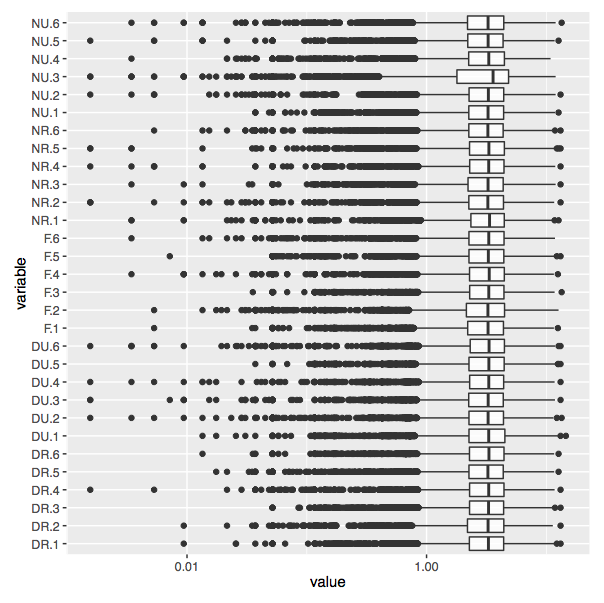
\includegraphics[width=\textwidth]{boxplotPW}
    \end{framed}
    \caption{Boxplot of the all 30 samples after betweenLaneNormalization normalization method. Since we only expect a handful of transcripts to show differential expression, we expect the samples to be mostly similar. It seems that the third replicate of NU may need to be removed. Other than that, there does not appear to be systematic differences in the samples after this normalization.}
    \label{fig:boxplotPW}
\end{figure}

After removing the third replicate of NU, we created an MDS plot to better understand the quality of the data (\citealt{limma}) (see Figure \ref{fig:mdsPW}).

\begin{figure}[H]
    \begin{framed}
    \centering
    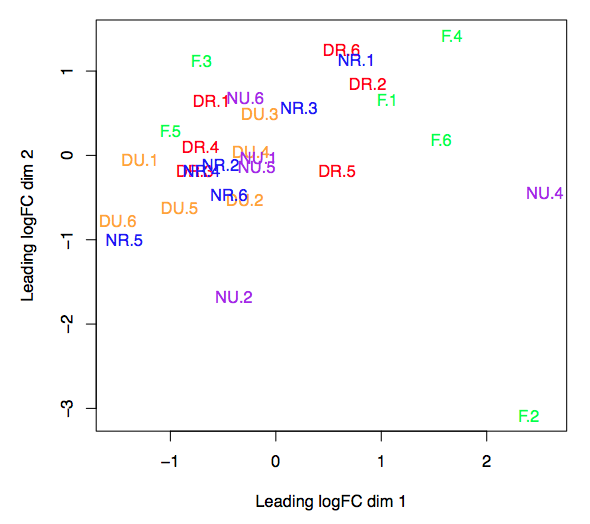
\includegraphics[width=\textwidth]{mdsPW}
    \end{framed}
    \caption{MDS plot of the 29 samples after removing the third replicate of the NU group.}
    \label{fig:mdsPW}
\end{figure}

We also examined scatterplot matrices of all pairwise combinations of the five treatment groups. These plots did not appear to show much of a difference in read counts in inter-replicates and as much of a similarity in read counts in intra-replicates as we saw previously with the soybean data back in Figure \ref{fig:L120scatter}.

\section{Highest quality replicates (Artificial Drumming groups)}

The visual tools of the boxplot, MDS, and scatterplot matrices made us believe that the two artificial drumming treament groups (DU and DR) were of the highest quality. As such, we subsetted the data to only consider these twelve samples for the time being. First, we converted the read counts to counts per million (cpm), because raw counts  do not account for differences in library sizes between samples. We then placed the cpm count values on a logarithmic scale. We also filtered the data: In general, genes should be discarded if they have zero probability of being expressed in all the samples for any of the treatments, and so we applied this rule of thumb (\citealt{edger}).

After filtering and normalizing on the twelve samples of interest (DU and DR), we then checked the quality again by creating a scatterplot matrix. As we stated earlier, the scatterplot matrices did not look too clean, and we see this even in the case of DU and DR (see Figure \ref{fig:scatMatPW}).

\begin{figure}[H]
    \begin{framed}
    \centering
    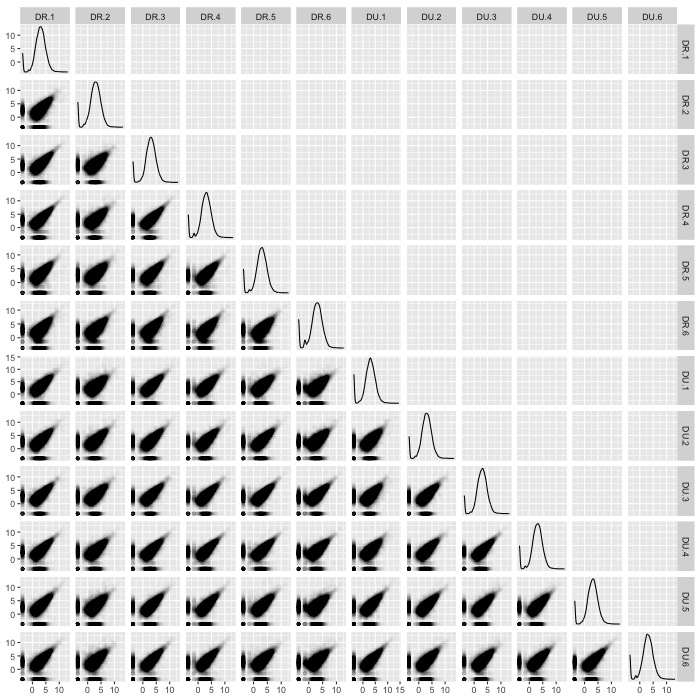
\includegraphics[width=\textwidth]{scatMatPW}
    \end{framed}
    \caption{Scatterplot matrix of the twelve samples of artificial drumming groups (DU and DR), where each individual scatterplot matrix compares two of the twelve samples. If the DU and DR treatment group samples are high quality, then we would expect replicates to have read counts centered on the diagonal x=y line, and non-relicates to deviate somewhat from the diagonal x=y line. We do not see this so clearly: The bottom-left 36 plots (non-replicates) do not appear much (if any) thicker around the x=y line than the other plots (replicates).}
    \label{fig:scatMatPW}
\end{figure}

\subsection{Differential expression analysis}

We performed significance testing on just the 12 samples of the treatment groups DU and DR, mostly following the recommended pre-processing protocol recommended in edgeR (\citealt{edger}). We then created single transcript plots (similar to what we did in Figures \ref{fig:indSBGenes1} and \ref{fig:indSBGenes2}) for the transcripts that were the most differentially expressed. The results of the top ten differentially expressed transcripts are shown below in Figure \ref{fig:degPW}.

\begin{figure}[H]
    \centering
    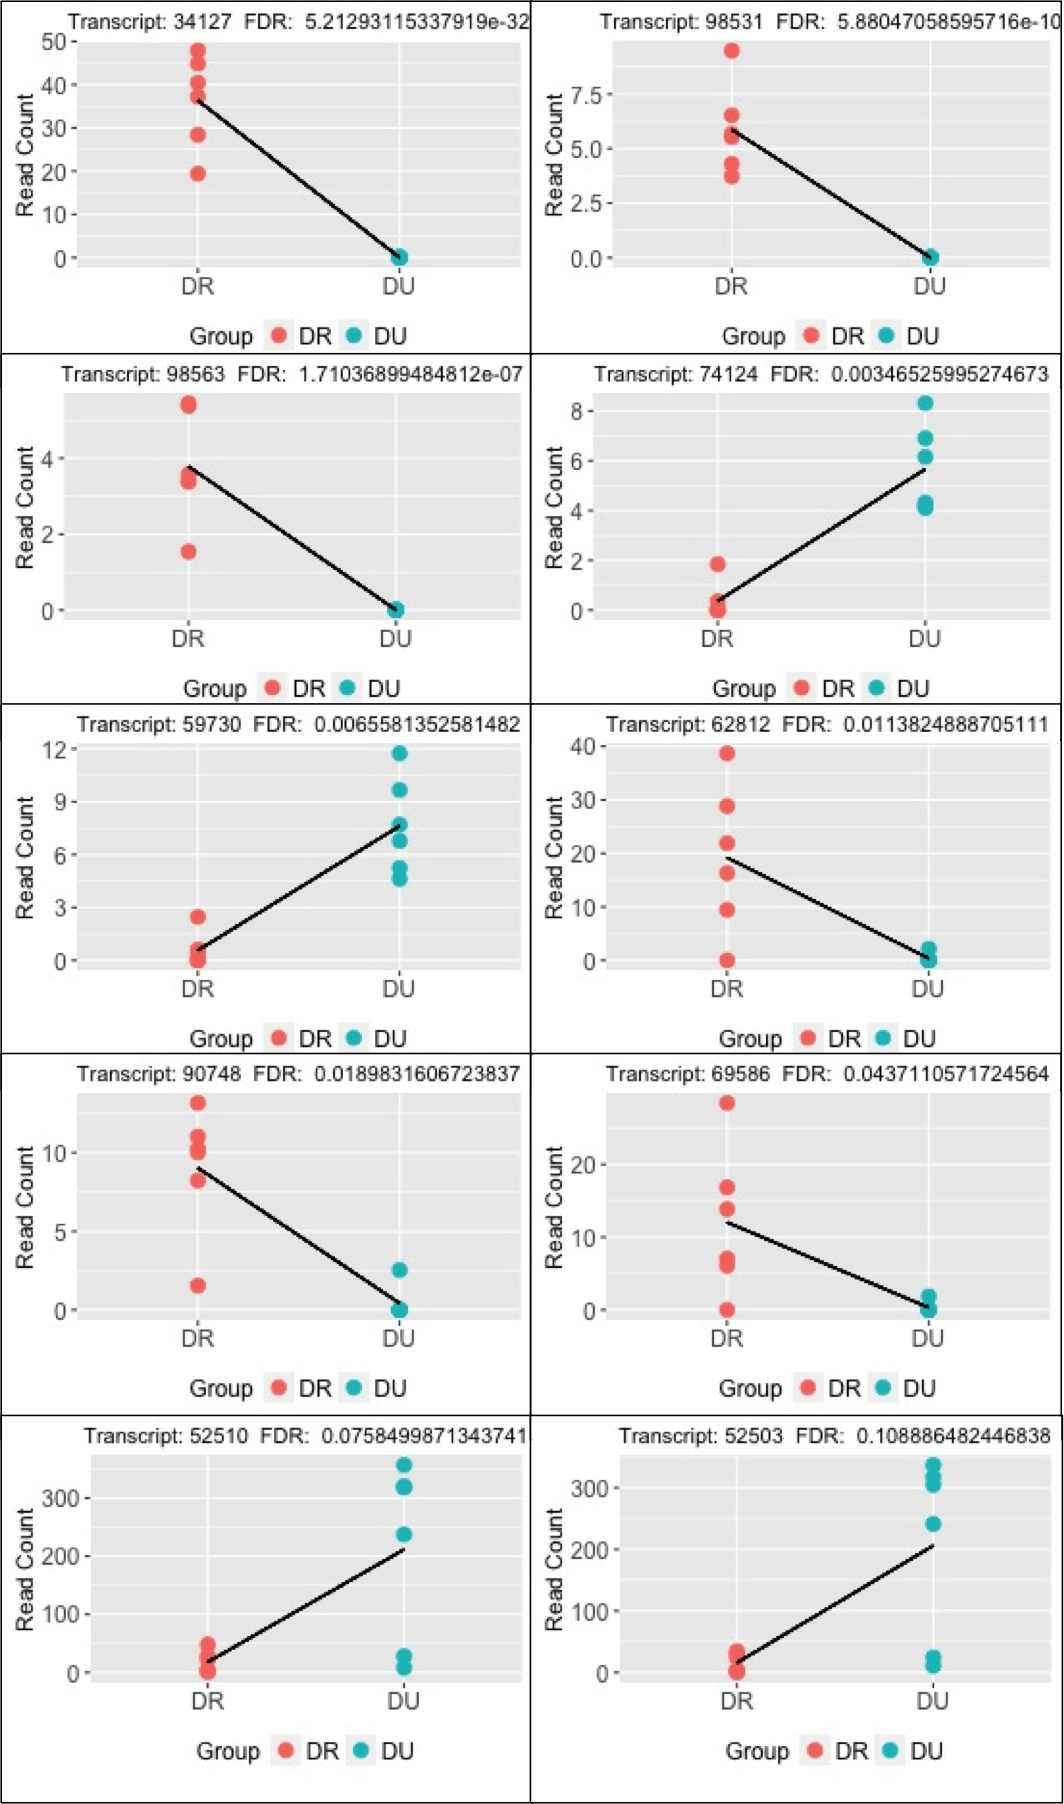
\includegraphics[width=0.9\textwidth]{degPW}
    \caption{The ten transcripts with the lowest FDR values after performing differential expression analysis using edgeR comparing the DU and DR groups. Each sample read count is represented as a dot and a black line connects the mean read counts from the two treatment groups. The differential expression can be visually verified; it appears that these transcripts did have significant differences in read counts between treatment groups.}
    \label{fig:degPW}
\end{figure}

\section{Future Avenues}

We have several avenues we could pursue to expand upon this work:

\begin{enumerate}
\item \textbf{Strengthen normalization}: The MDS plot, scatterplot matrices, and parallel coordinate plots from clustering analysis did not appear as clean in the paper wasp data as they did for soybean data. One method we can approach is a more robest normalization process as outline in the RUVseq package (\citealt{ruvseq}). Within this approach, there are three possible directions in which a handful of "negative control transcripts" must be used.

\begin{enumerate}
\item \textbf{Housekeeping transcripts}: In this approach, we would use a small number of robust transcripts with known quantities that do not change much from one treatment to another. For the \textit{Polistes fuscatus} transcriptome, there are a small number of known transcripts for this purpose (such as actin, rp49, and S8), although their usefulness is dubious as their quantity can vary considerably across different experimental conditions.
\item \textbf{Internal control transcripts}: In this approach, we obtain an "in-silico empirical" set of negative control transcripts by examining the properties of the transcripts within the data itself. This approach is ideal if we cannot obtain a set of negative control transcripts elsewhere.
\item \textbf{Spike-in controls}: In this approach, a known concentration of RNA transcripts are applied. As such, they can be advantageous to endogenous controls. However, we have yet to determine if the RNA-sequencing for this data had employed spike-in controls. 
\end{enumerate}

\item \textbf{Map to genome}: We have thusfar examined the transcript read counts after the reads were mapped to the transcriptome from the same species (\citealt{pw19}). We could also consider examining the genome read counts by mapping the reads to the genome of a similar species.

\item \textbf{Permutation testing}: Although the top differentially expressed transcripts between DU and DR looked promising (in Figure \ref{fig:degPW}), will also develop permutation testing for this type of visual analysis of differentially expressed transcripts. Namely, we can create permutations where the sample names (DU.1, DU.2, ..., DR.6) are randomly assigned to columns in the data. After that, we can rerun the edgeR process on this falsely-named data, determine the new set of differentially expressed transcripts, and examine this new set visually with the same plots as in Figure \ref{fig:degPW}. At this point, we can create a lineup of the most statistically-significantly differentially expressed transcripts from the real dataset and from two permuted datasets. This would create a "triplet plot", where the location of the actual data plot is randomized amongst the two permuted data plots. If the actual data plot can be distinguished from the permuted data plots, then we have evidence that the differential expression we found was more due to treatment differences than other differences. To accomplish this, we plan on using the \pkg{nullabor} package (\citealt{nullabor}).

\item \textbf{Render plotting interactive}: It would be useful to allow for the permutation testing visualization tools to have an interactive element. For example, users could quickly glance through the triplet plots of the top differentially expressed transcripts to discover if there are any transcripts that appear suspcious. Or, they could quickly rerun the permutation testing on a different set of treatment groups of interest.

\end{enumerate}

\section{Conclusions}

The paper wasp data did not respond as well as the soybean data did to the visual tools for RNA-sequencing clustering analysis (which we did not explicitly show in this thesis proposal). This may be due to the fact that the soybean replicates were clones, whereas the wasp replicates were not clones. Moreover, the soybean data is more controlled than the wild paper wasps. It could also be due to us using transcript read counts for the paper wasp data, while we used gene read counts for the soybean data. While there is only neglible overlap between transcripts, there is no longer independence as multiple transcripts can map to the same gene.

We have preliminary plotting tools for RNA-sequencing signficance testing analysis. We could see that the top differentially expressed transcripts did appear as we would expect in Figure \ref{fig:degPW}. We can now expand upon this by creating interactive permutation testing visualizations of these differentially expressed transcripts.

\section{Acknowledgments}

\textbf{\textcolor{Red}{What should I Put here? We would like to thank Dr. Jennifer M. Jandt for sharing the \textit{Polistes fuscatus} RNA-sequencing data.}}

\chapter{Timeline}
\label{sec:timeline}

\section{Completed}

\begin{tabular}{|p{3cm}|p{8cm}|p{3cm}|}
 \hline
 \textbf{Product} & \textbf{Description} & \textbf{Date} \\ 
 \hline
 R package & First release of \pkg{ggenealogy}, which provides visualization tools for genealogical datasets & March 2015 \\
 \hline
 Presentation & Presented \pkg{ggenealogy} at JSM & August 2015 \\
 \hline
 Award & Student paper award at ASA Statistical Computing and Graphics Section & August 2015 \\
 \hline
\end{tabular}

\section{Scheduled deliverables}

\begin{tabular}{|p{3cm}|p{8cm}|p{3cm}|}
 \hline
 \textbf{Product} & \textbf{Description} & \textbf{Date} \\ 
 \hline
 R package & Second release of \pkg{ggenealogy} package, which provides visualization tools for genealogical datasets & May 2016 \\
 \hline
 Paper & Submit \pkg{ggenealogy} paper to JSS & May 2016 \\
 \hline
 R package & First release of package that provides visualization tools for RNA-sequencing datasets & TBD \\
 \hline
 Paper & Submit paper about package that provides visualization tools for RNA-sequencing & TBD \\
 \hline
\end{tabular}

\section{Other work}

\begin{tabular}{|p{3cm}|p{8cm}|p{3cm}|}
 \hline
 \textbf{Product} & \textbf{Description} & \textbf{Date} \\ 
 \hline
 R package & First release of ePort & July 2016 \\
 \hline
\end{tabular}

\bibliography{myThesis}

\end{document}
